\section{Generative AI e NLP}
\label{sec:genai_nlp}
%
\begin{frame}[t] \frametitle{Machine Learning}
\framesubtitle{Schema di \emph{workflow} semplificato}
	\begin{minipage}[t]{\textwidth}
		\vspace{-.7cm}
		\begin{figure}
			\centering
			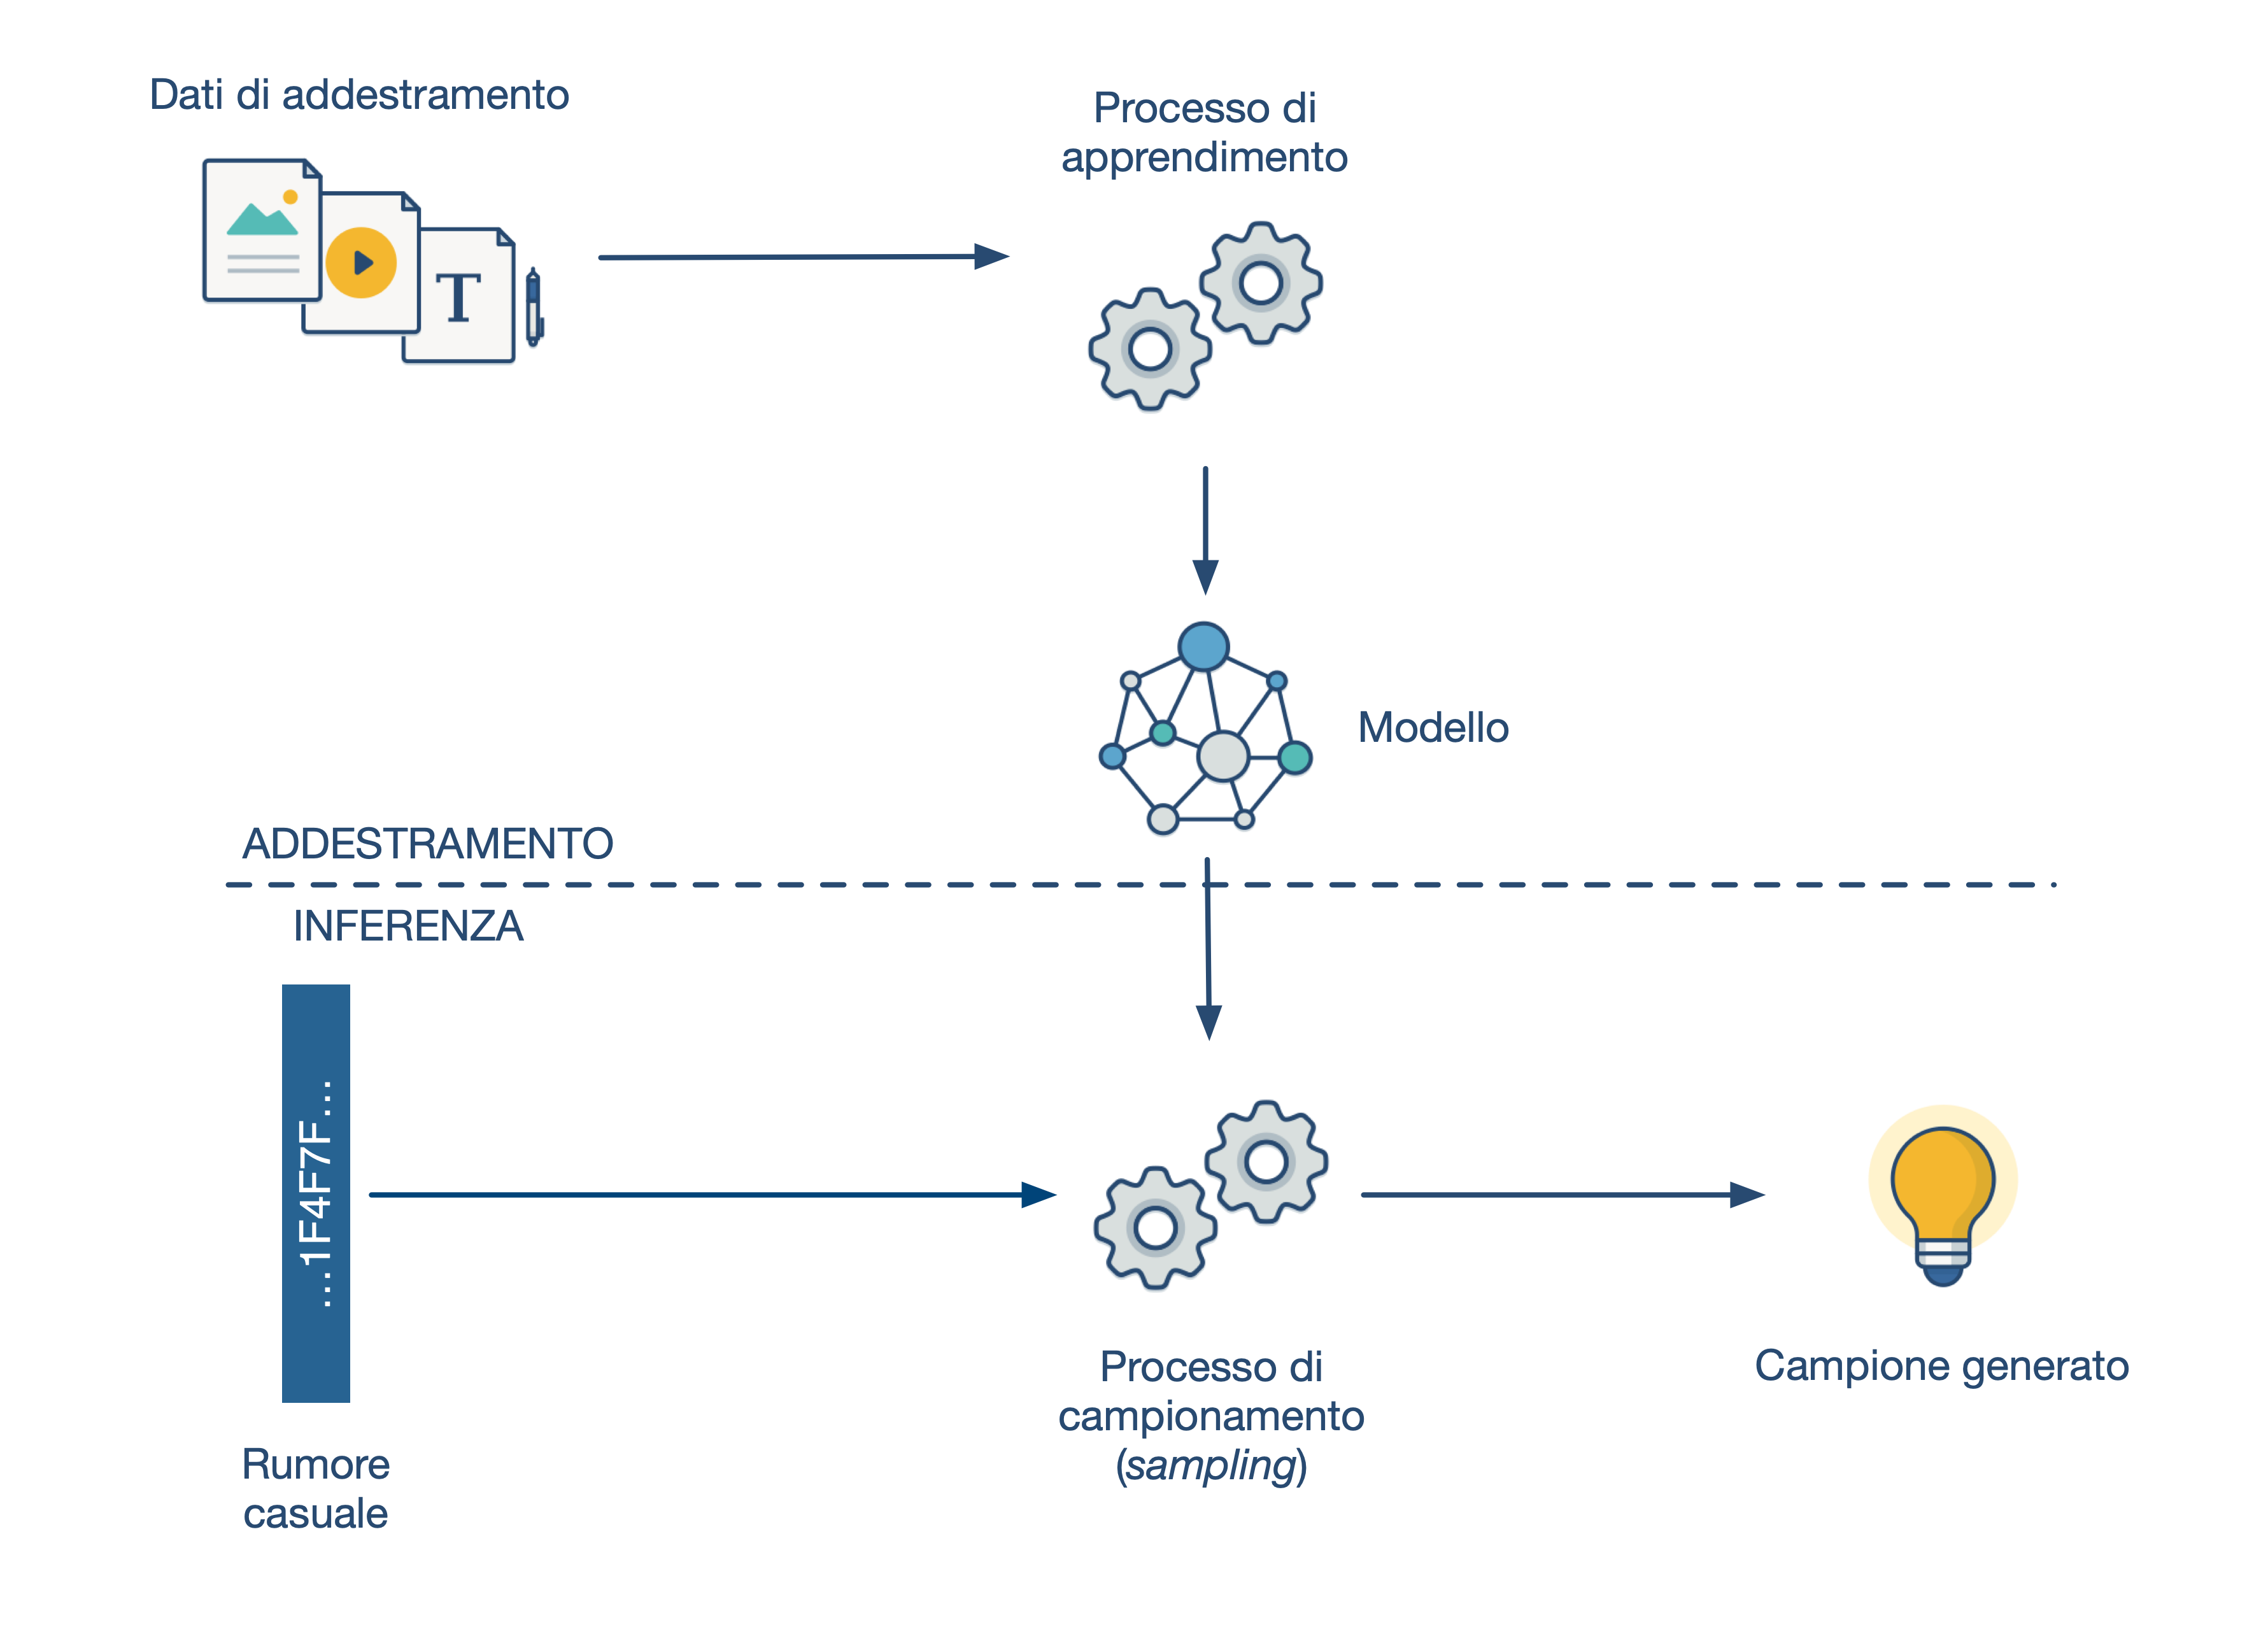
\includegraphics[width=.8\textwidth]{Generative-model-1.png}
		\end{figure}
        \begin{flushright}
            \vspace*{-10pt}
            {\tiny\textit{\textcopyright Simone Scannapieco}}
        \end{flushright}
	\end{minipage}
\end{frame}
%
\begin{frame}[t] \frametitle{Modelli generativi}
\framesubtitle{Schema di \emph{workflow} semplificato}
	\begin{minipage}[t]{\textwidth}
		\vspace{-.7cm}
		\begin{figure}
			\centering
			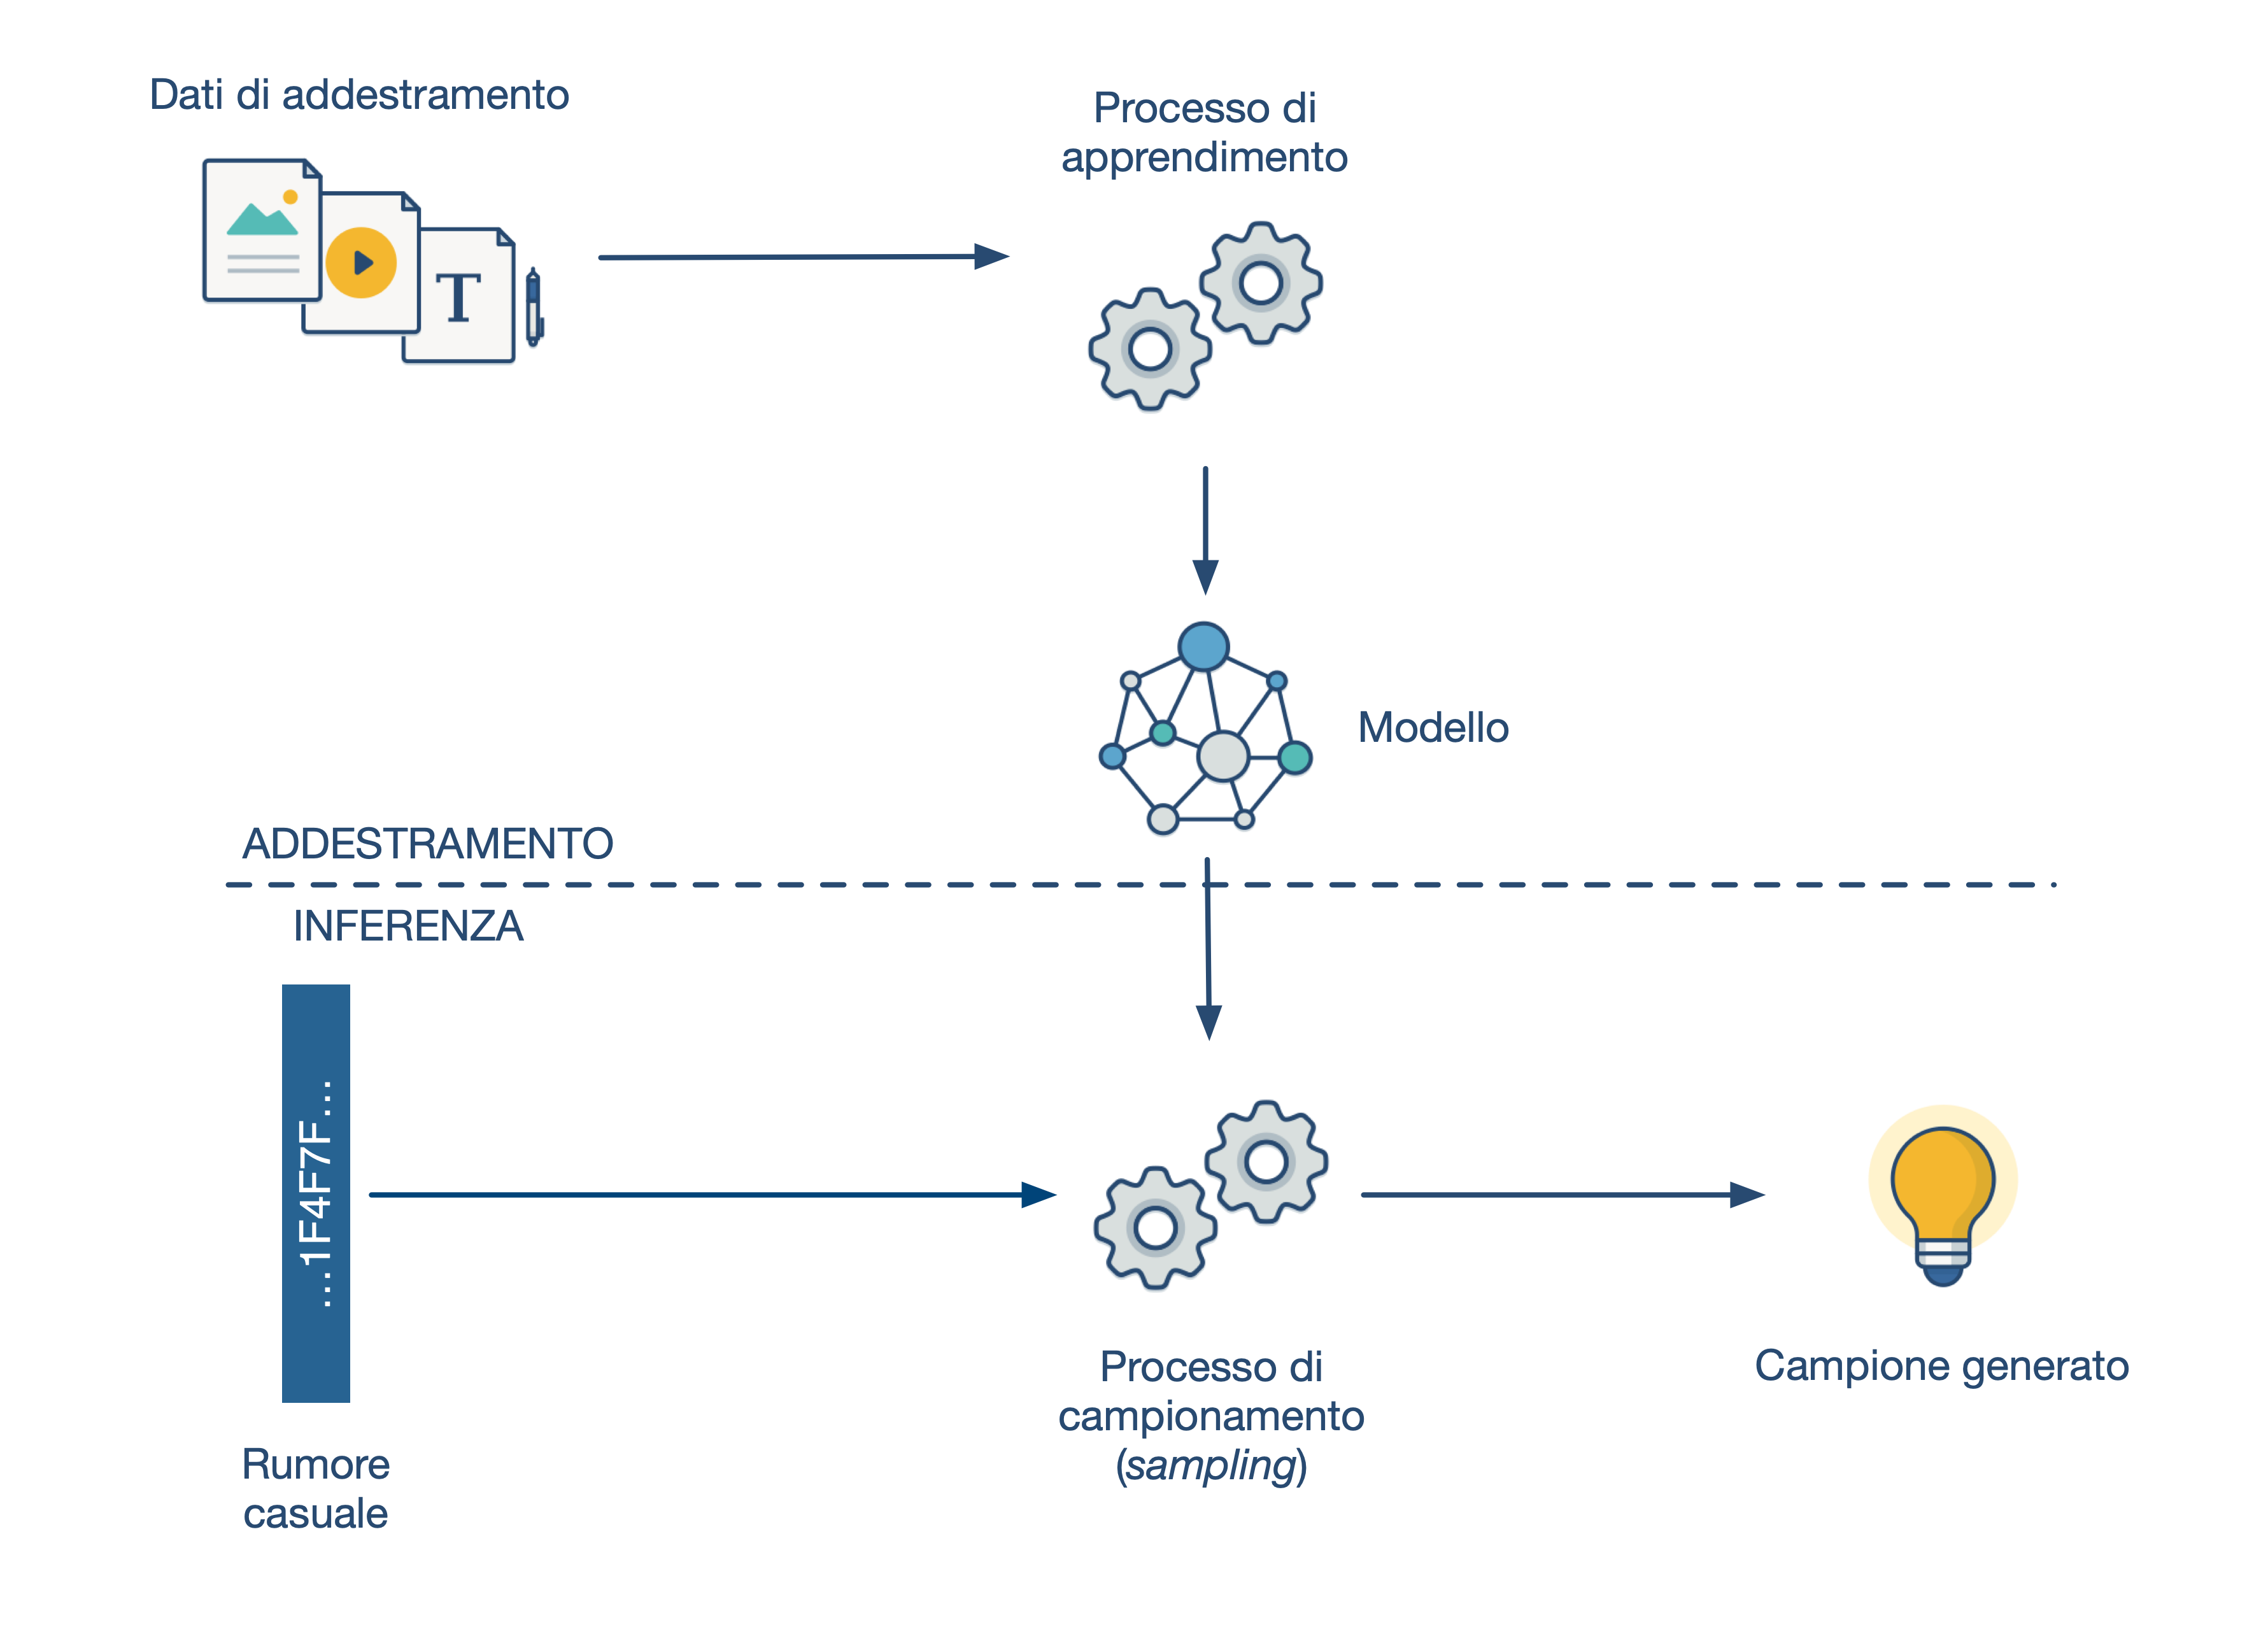
\includegraphics[width=.8\textwidth]{Generative-model-1.png}
		\end{figure}
        \begin{flushright}
            \vspace*{-10pt}
            {\tiny\textit{\textcopyright Simone Scannapieco}}
        \end{flushright}
		\vspace{-.3cm}
		\begin{itemize}[leftmargin=10pt,align=right]
			\item[\alert{\faArrowCircleRight}] Addestramento automatico prevalentemente \alert{non supervisionato}
		\end{itemize}
	\end{minipage}
\end{frame}
%
\begin{frame}[t] \frametitle{Modelli generativi}
\framesubtitle{Schema di \emph{workflow} semplificato - esempio MNIST}
{\footnotesize
	\begin{minipage}[t]{\textwidth}
		\vspace{-.7cm}
		\begin{figure}
			\centering
			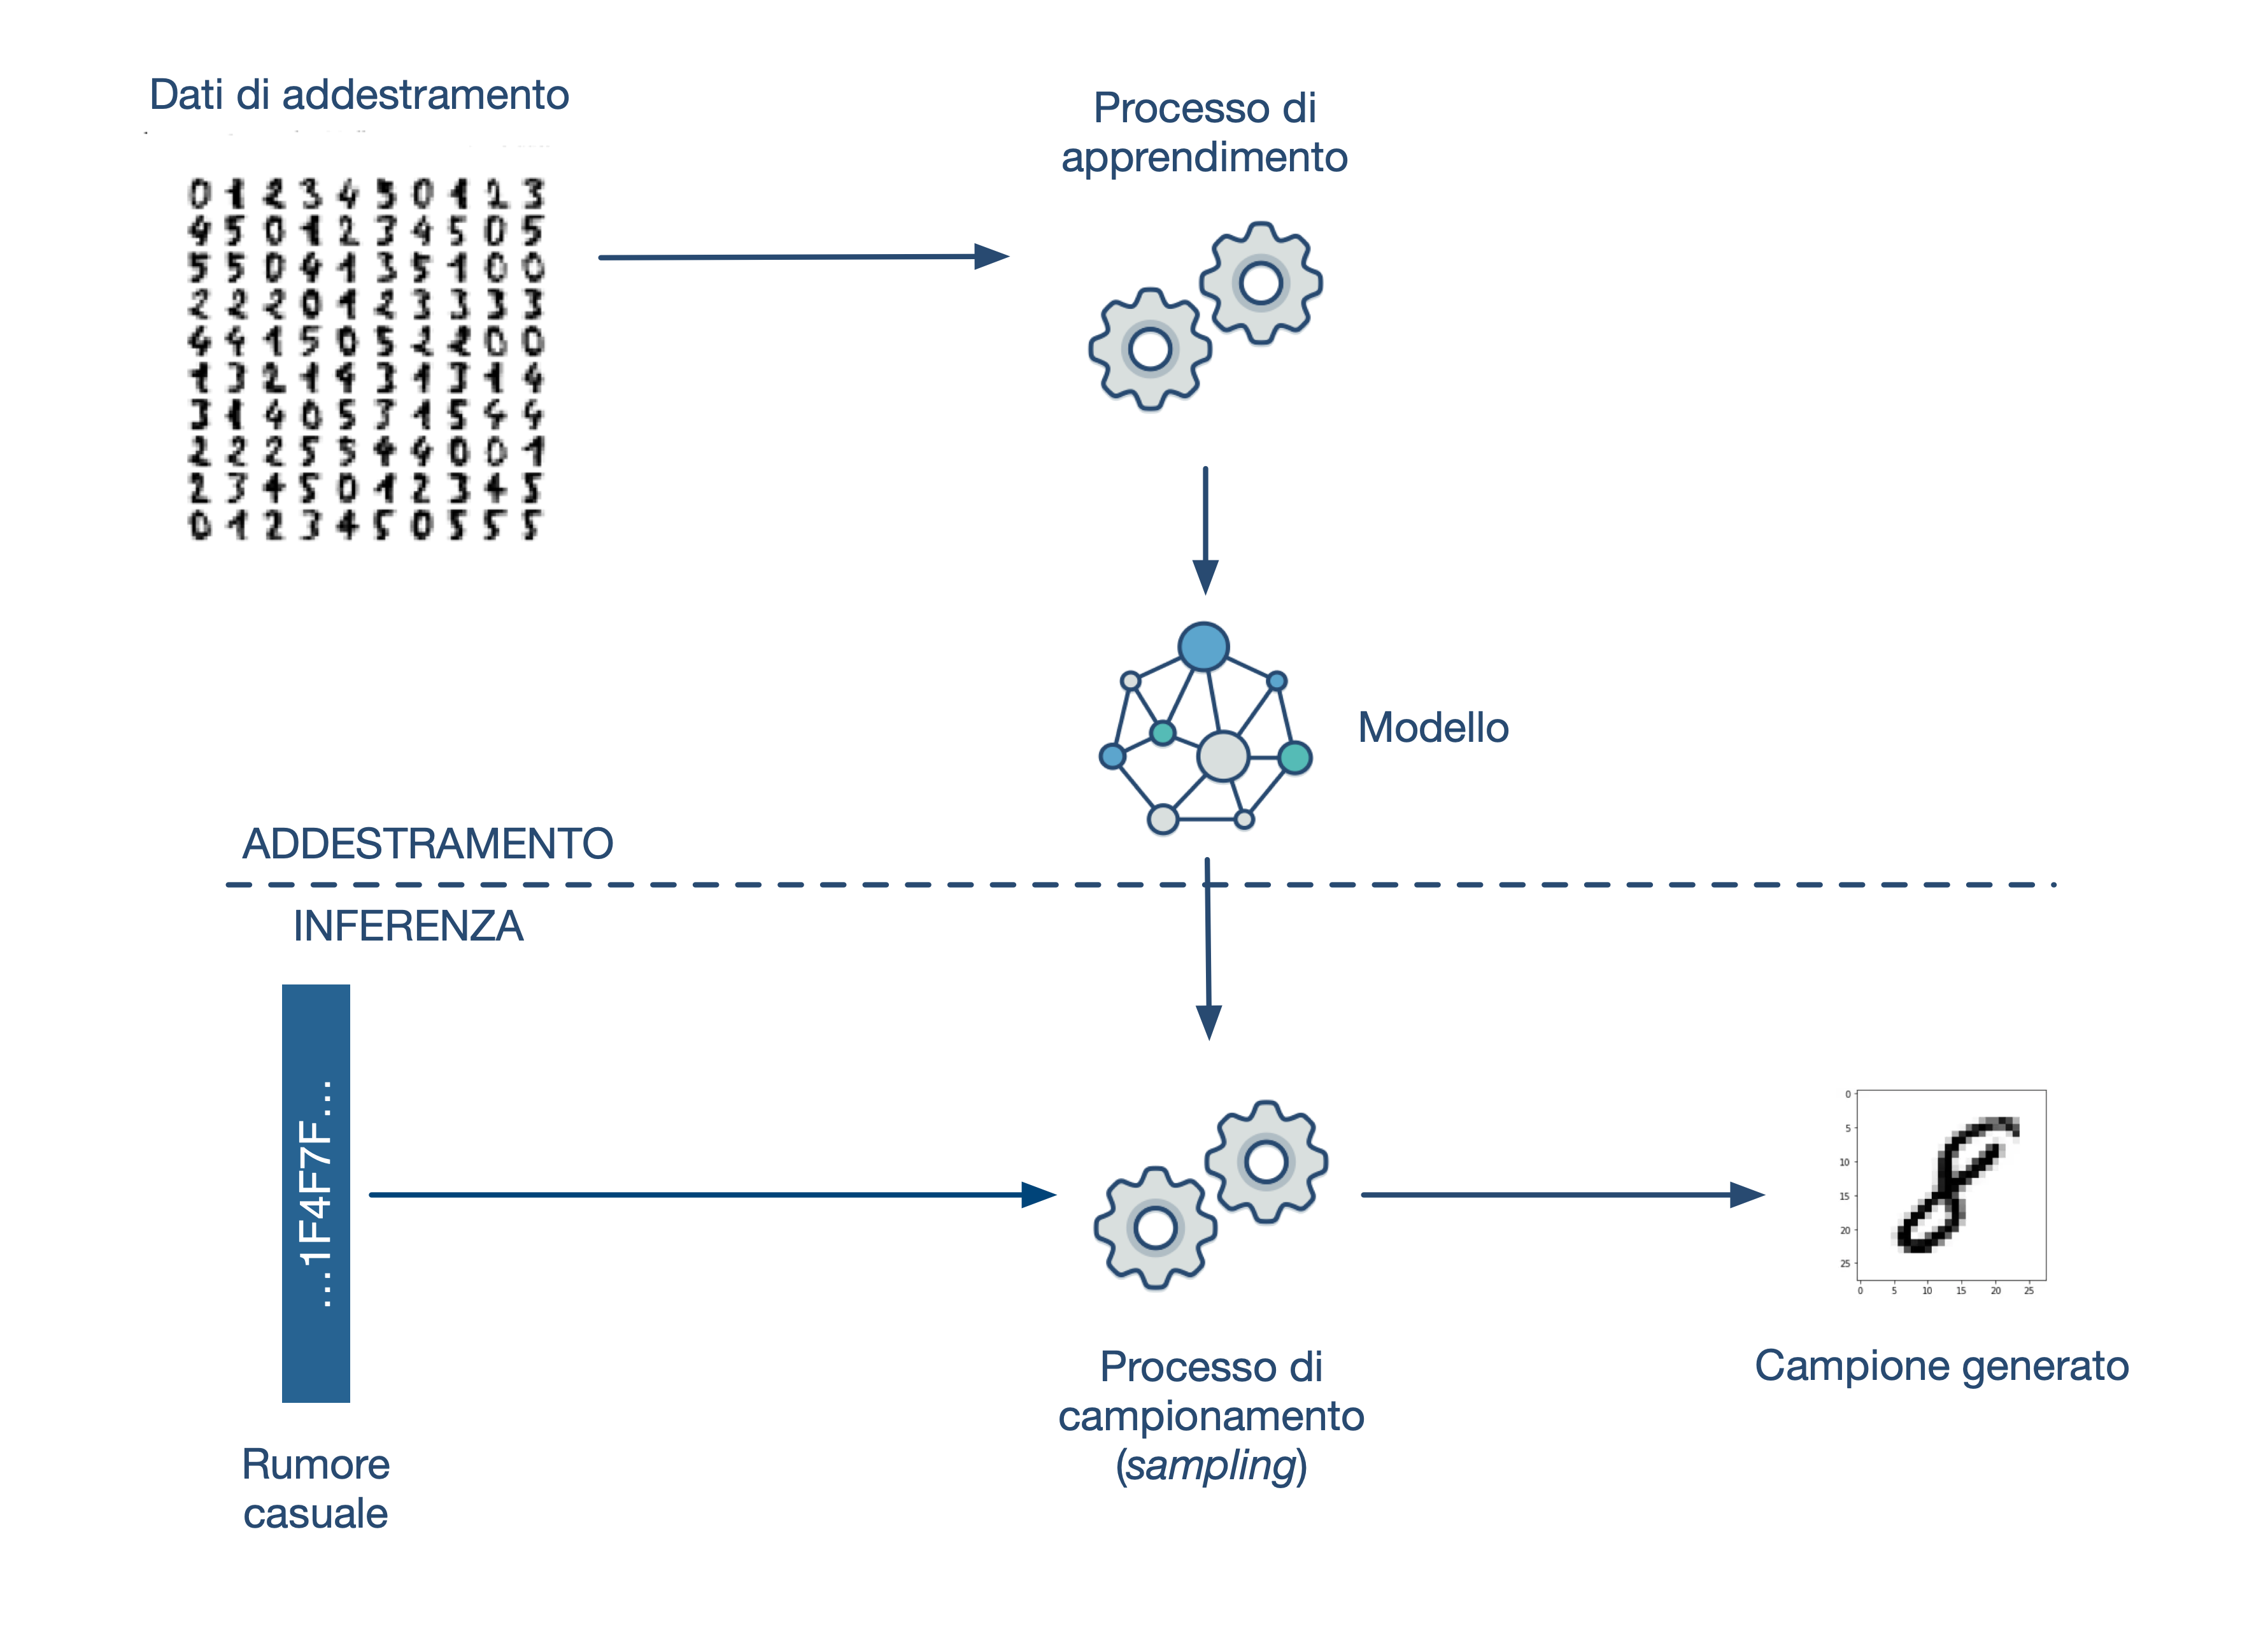
\includegraphics[width=.8\textwidth]{Generative-model-2.png}
		\end{figure}
		\begin{flushright}
			 \vspace*{-10pt}
            {\tiny\textit{\textcopyright Simone Scannapieco, Nischal Madiraju}}
		\end{flushright}
	\end{minipage}
}
\end{frame}
%
\begin{frame}[t] \frametitle{GENAI}
\framesubtitle{Sfera di interesse}
	\begin{itemize}[leftmargin=10pt,align=right]
		\onslide<1->\item[\alert{\faArrowCircleRight}] Definita la nuova era della AI
		\onslide<2->\item[\alert{\faArrowCircleRight}] Tre ambiti fondamentali
		\begin{enumerate}[leftmargin=10pt,align=right]
			\onslide<3->\item[\circled{alerted text.fg}{white}{1}]Generazione di testi
			\onslide<4->\item[\circled{alerted text.fg}{white}{2}] Generazione di codice
			\onslide<5->\item[\circled{alerted text.fg}{white}{3}] Generazione di contenuti multimodali (\alert{\textit{diffusion}})
		\end{enumerate}
		\onslide<6->\item[\alert{\faArrowCircleRight}] Ci focalizziamo su \circled{alerted text.fg}{white}{1}
	\end{itemize}
\end{frame}

\begin{frame}[t] \frametitle{GENAI}
\framesubtitle{Cronistoria architetturale}
{\scriptsize
\only<1>{
	\begin{figure}[ht]
		\begin{minipage}[b]{0.95\linewidth}
			\centering
			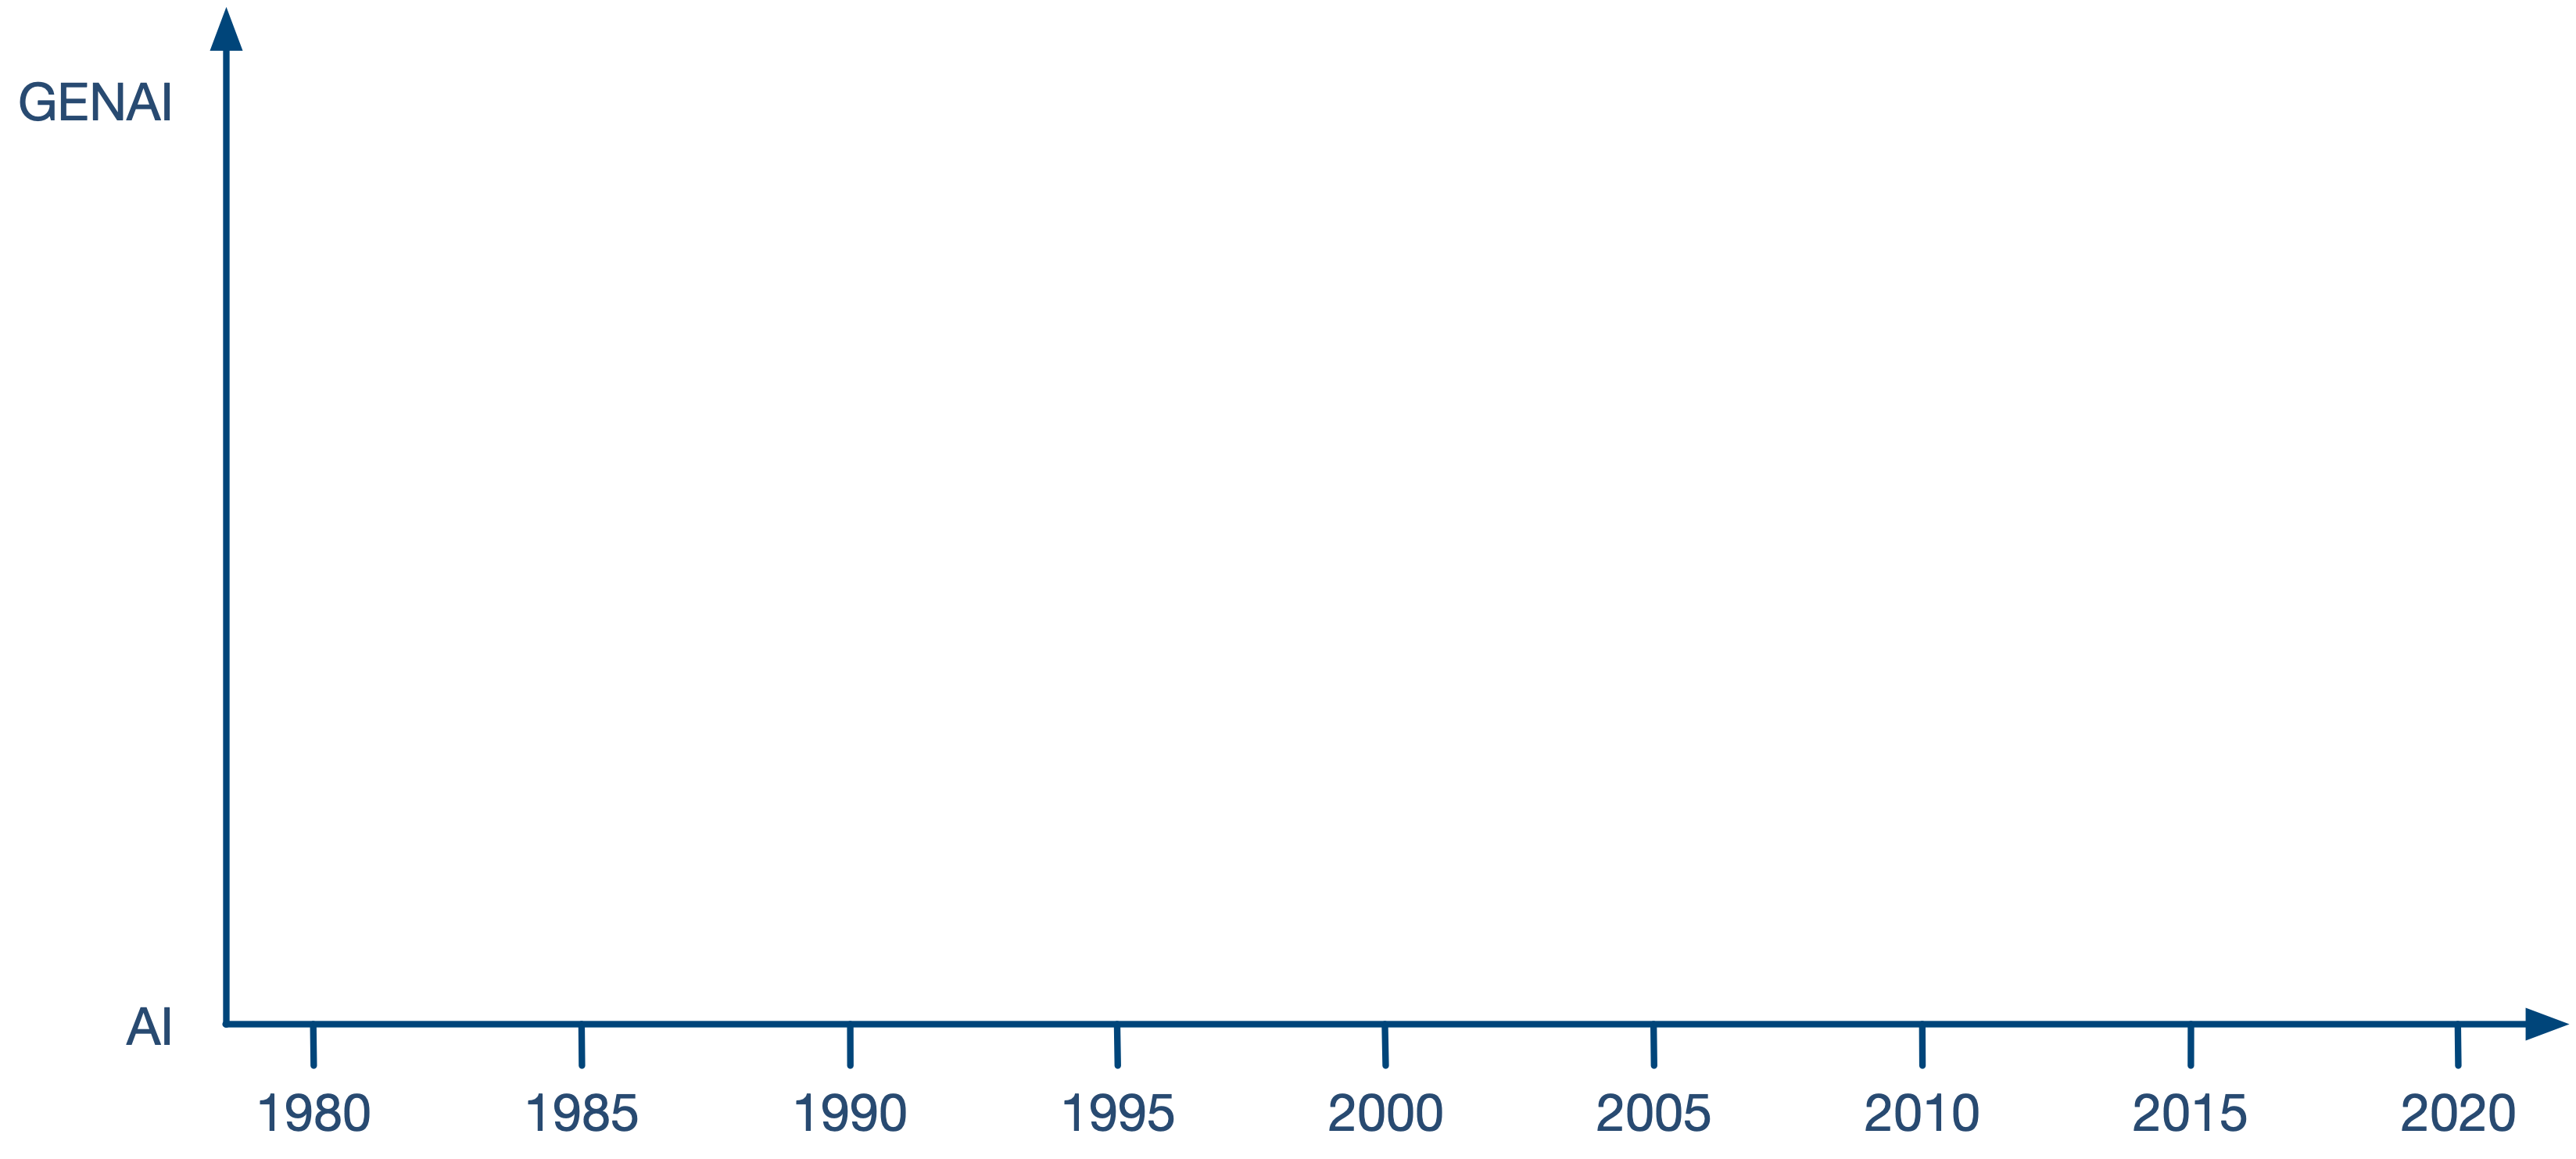
\includegraphics[width=\textwidth]{AI-GENAI.png}
		\end{minipage}
	\end{figure}
}
	\only<2>{
	\begin{figure}[ht]
		\begin{minipage}[b]{0.95\linewidth}
			\centering
			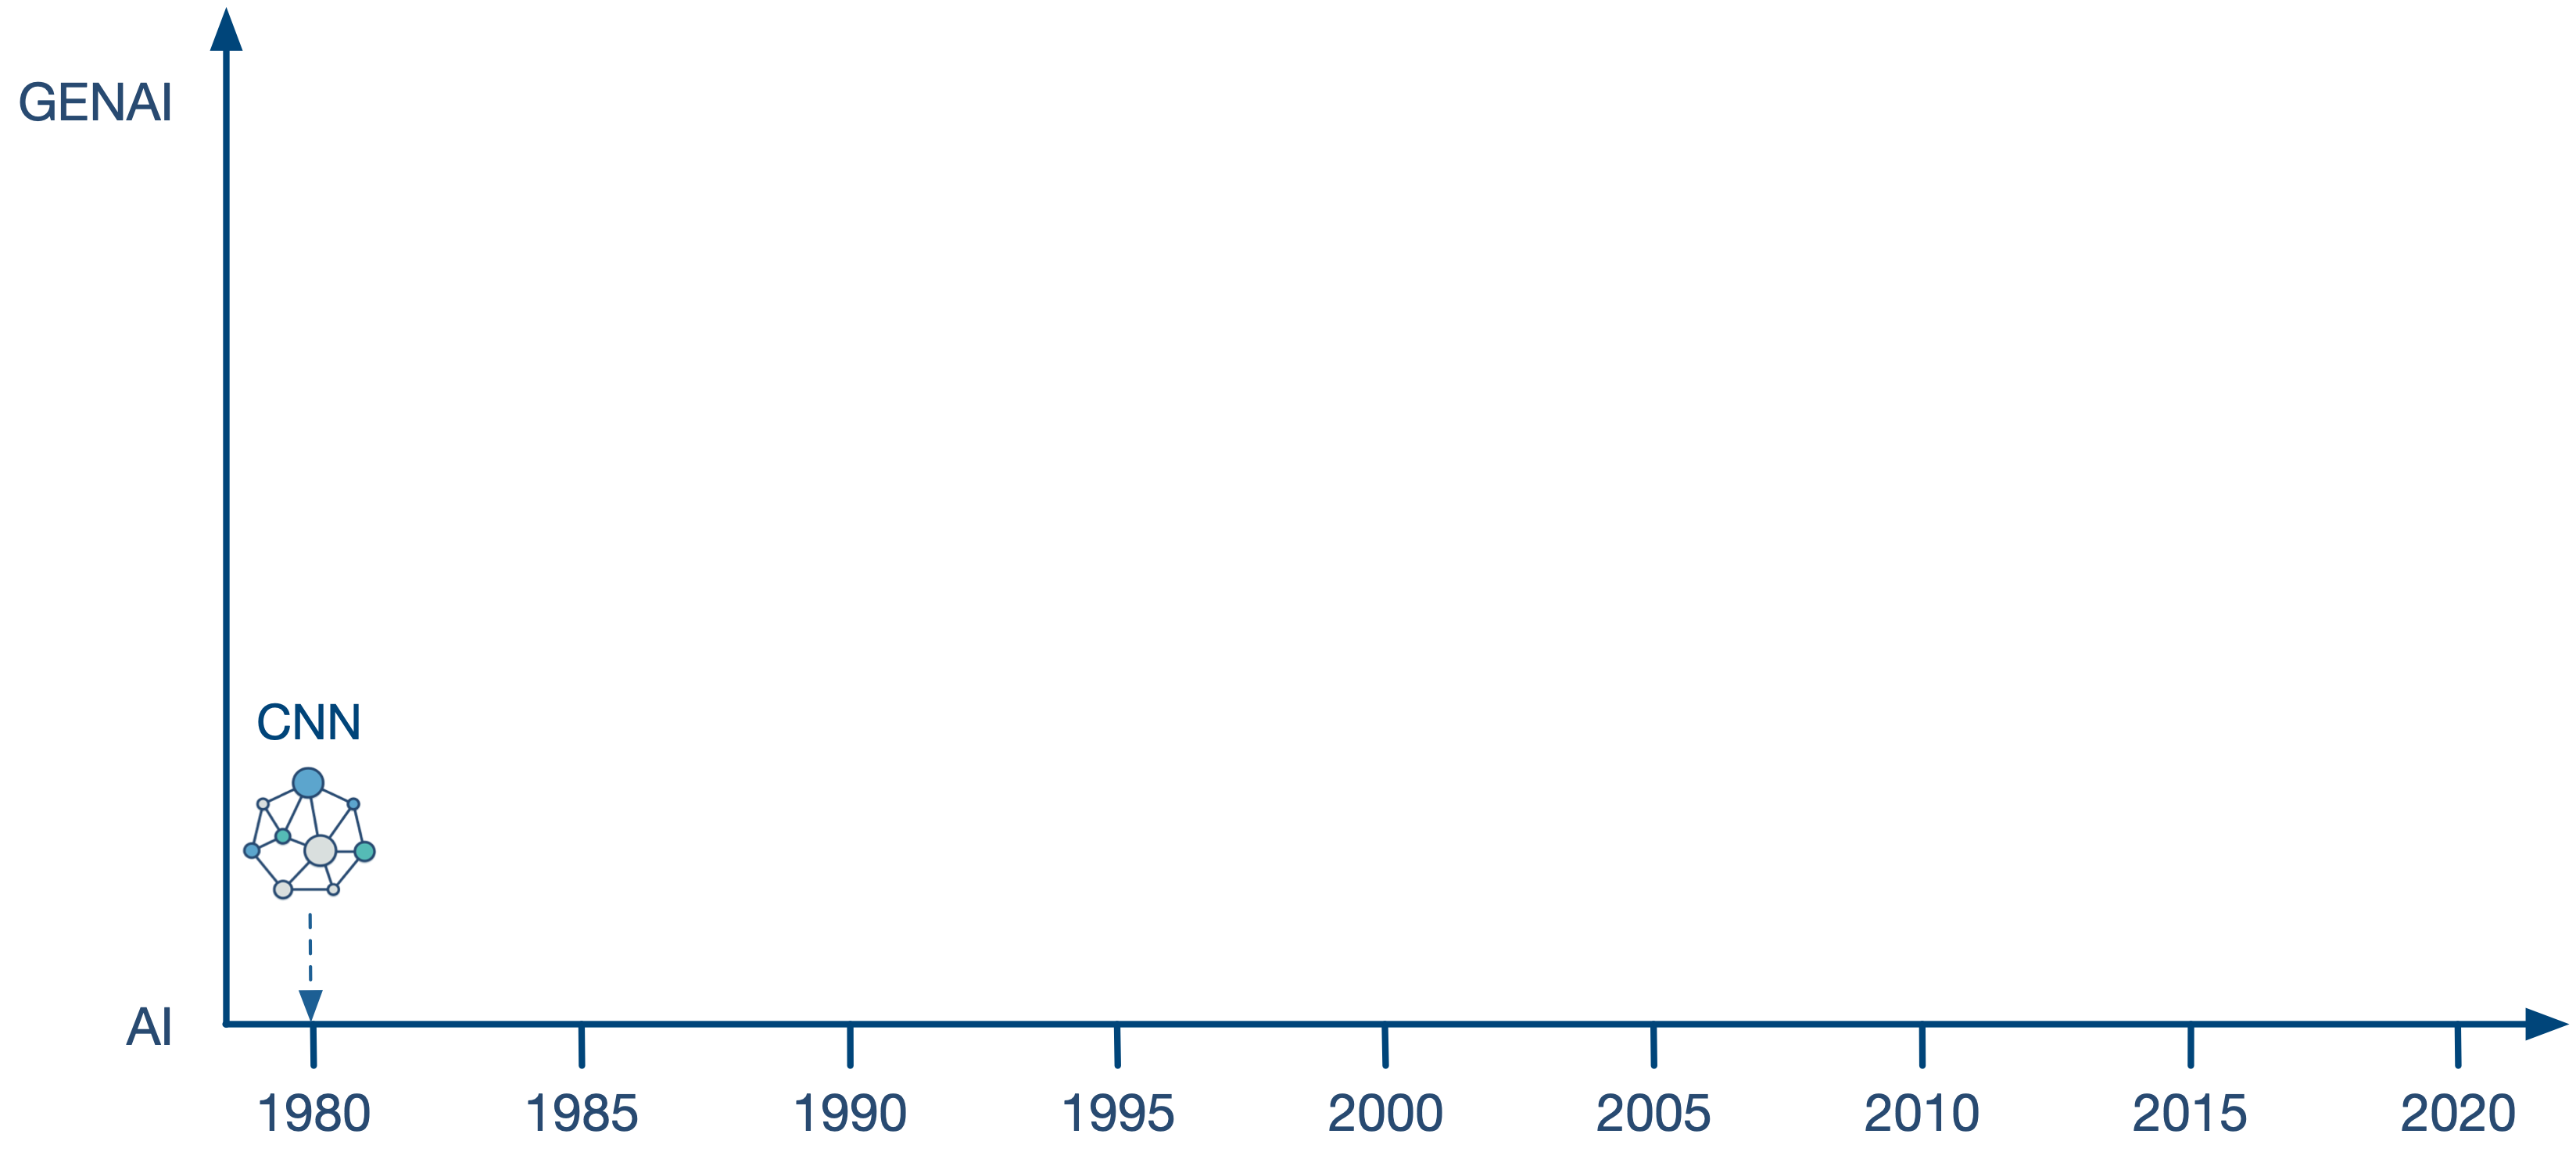
\includegraphics[width=\textwidth]{AI-GENAI-CNN.png}
		\end{minipage}
	\end{figure}
}
	\only<3>{
	\begin{figure}[ht]
		\begin{minipage}[b]{0.95\linewidth}
			\centering
			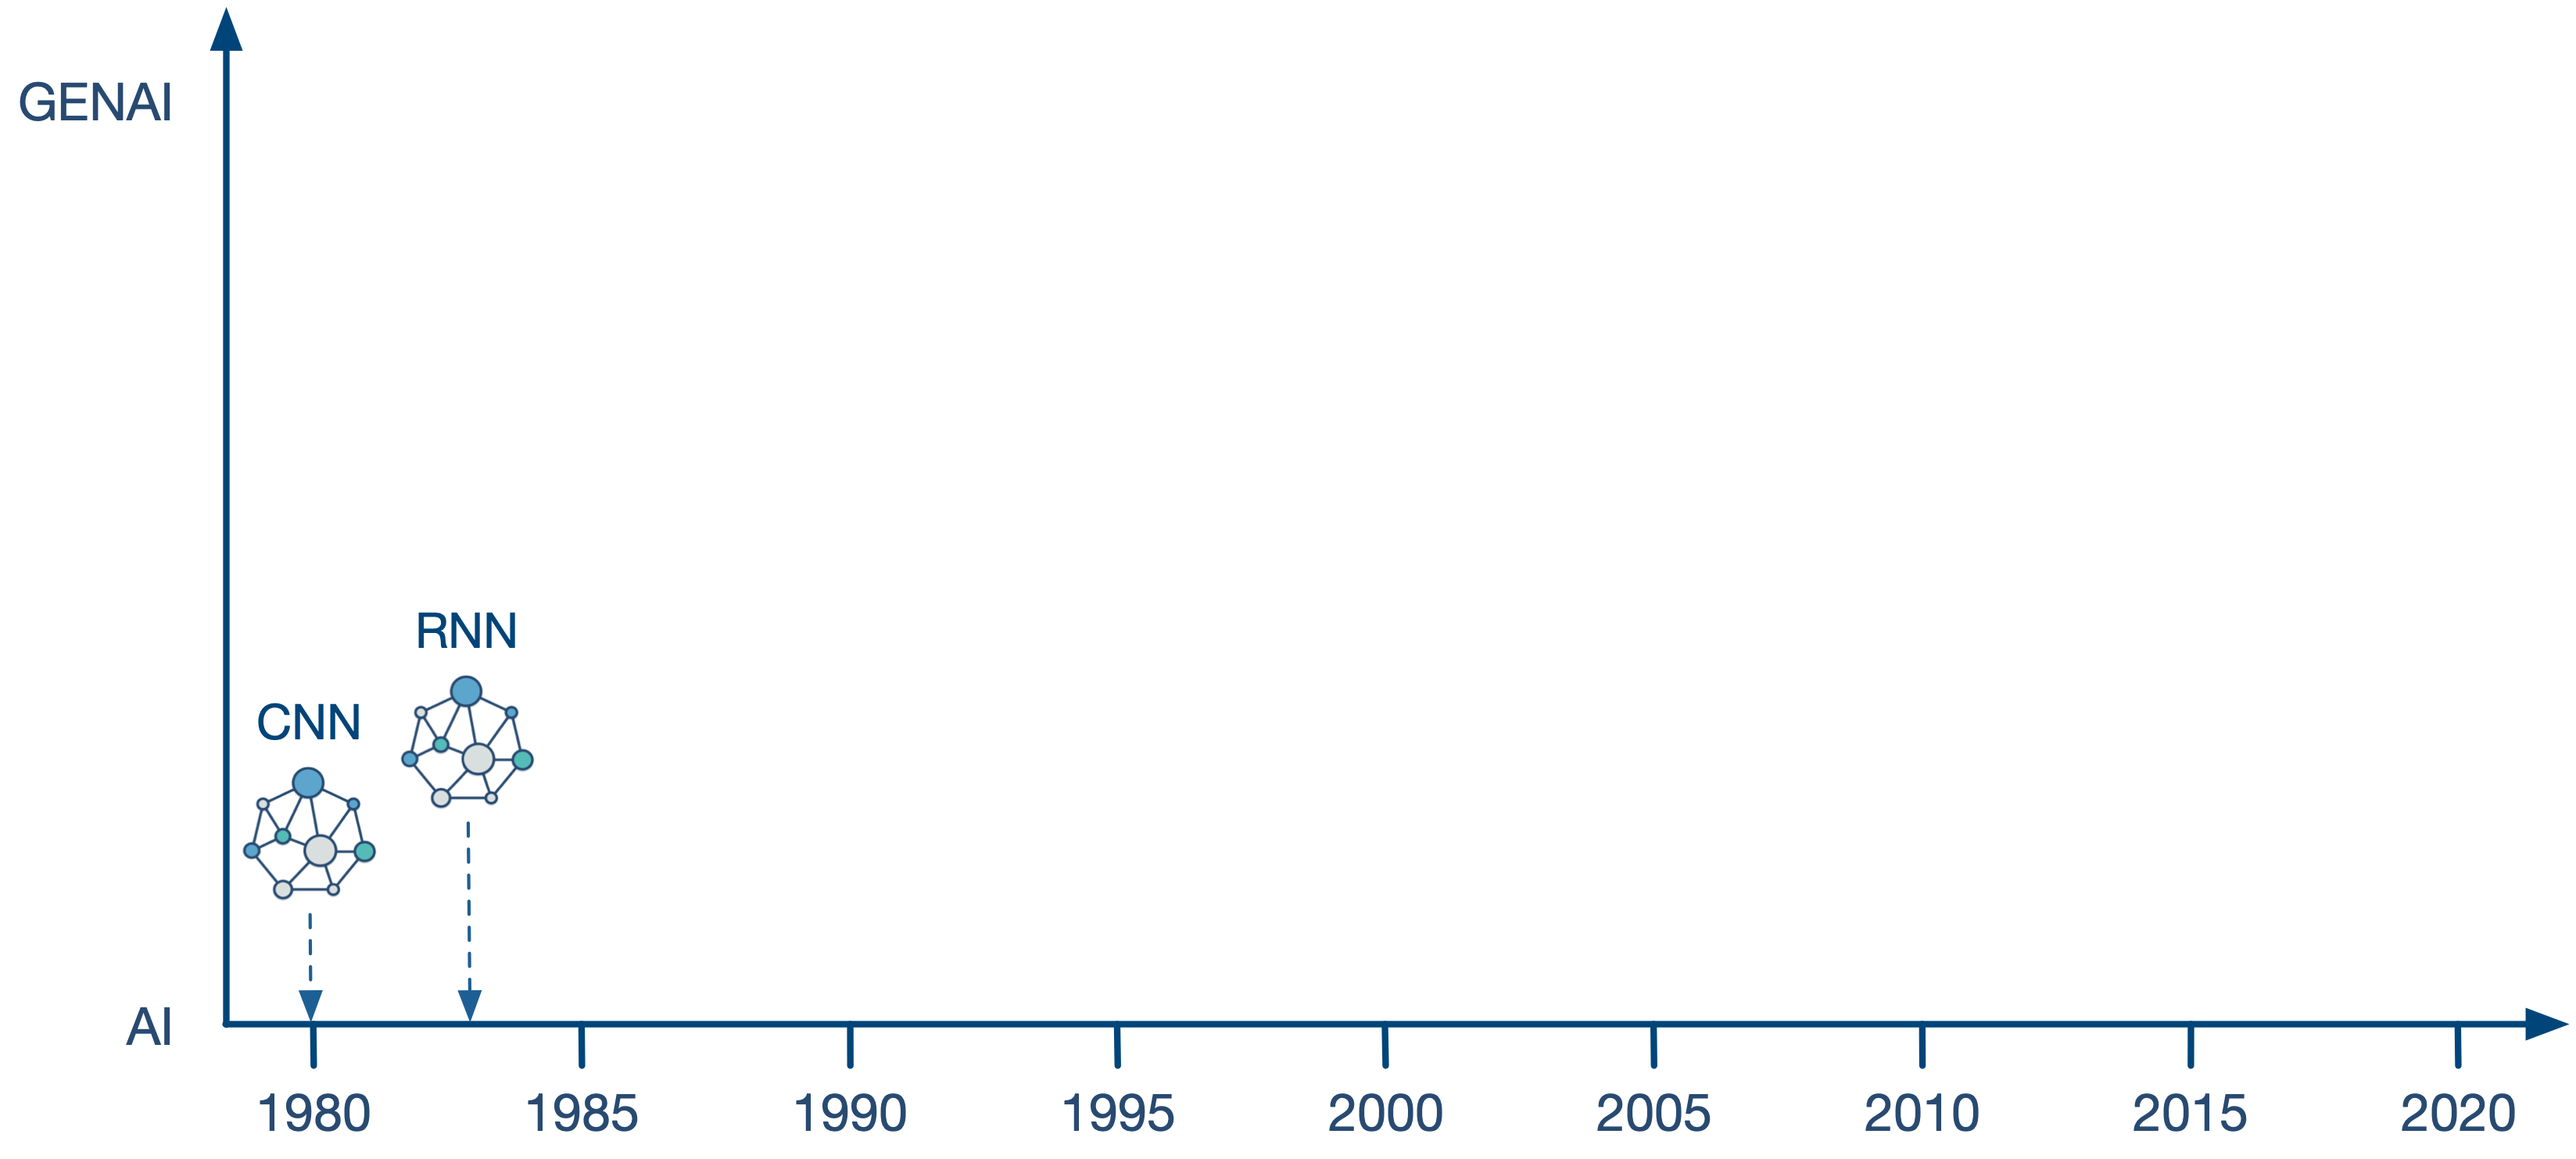
\includegraphics[width=\textwidth]{AI-GENAI-RNN.png}
		\end{minipage}
	\end{figure}
}
	\only<4>{
	\begin{figure}[ht]
		\begin{minipage}[b]{0.95\linewidth}
			\centering
			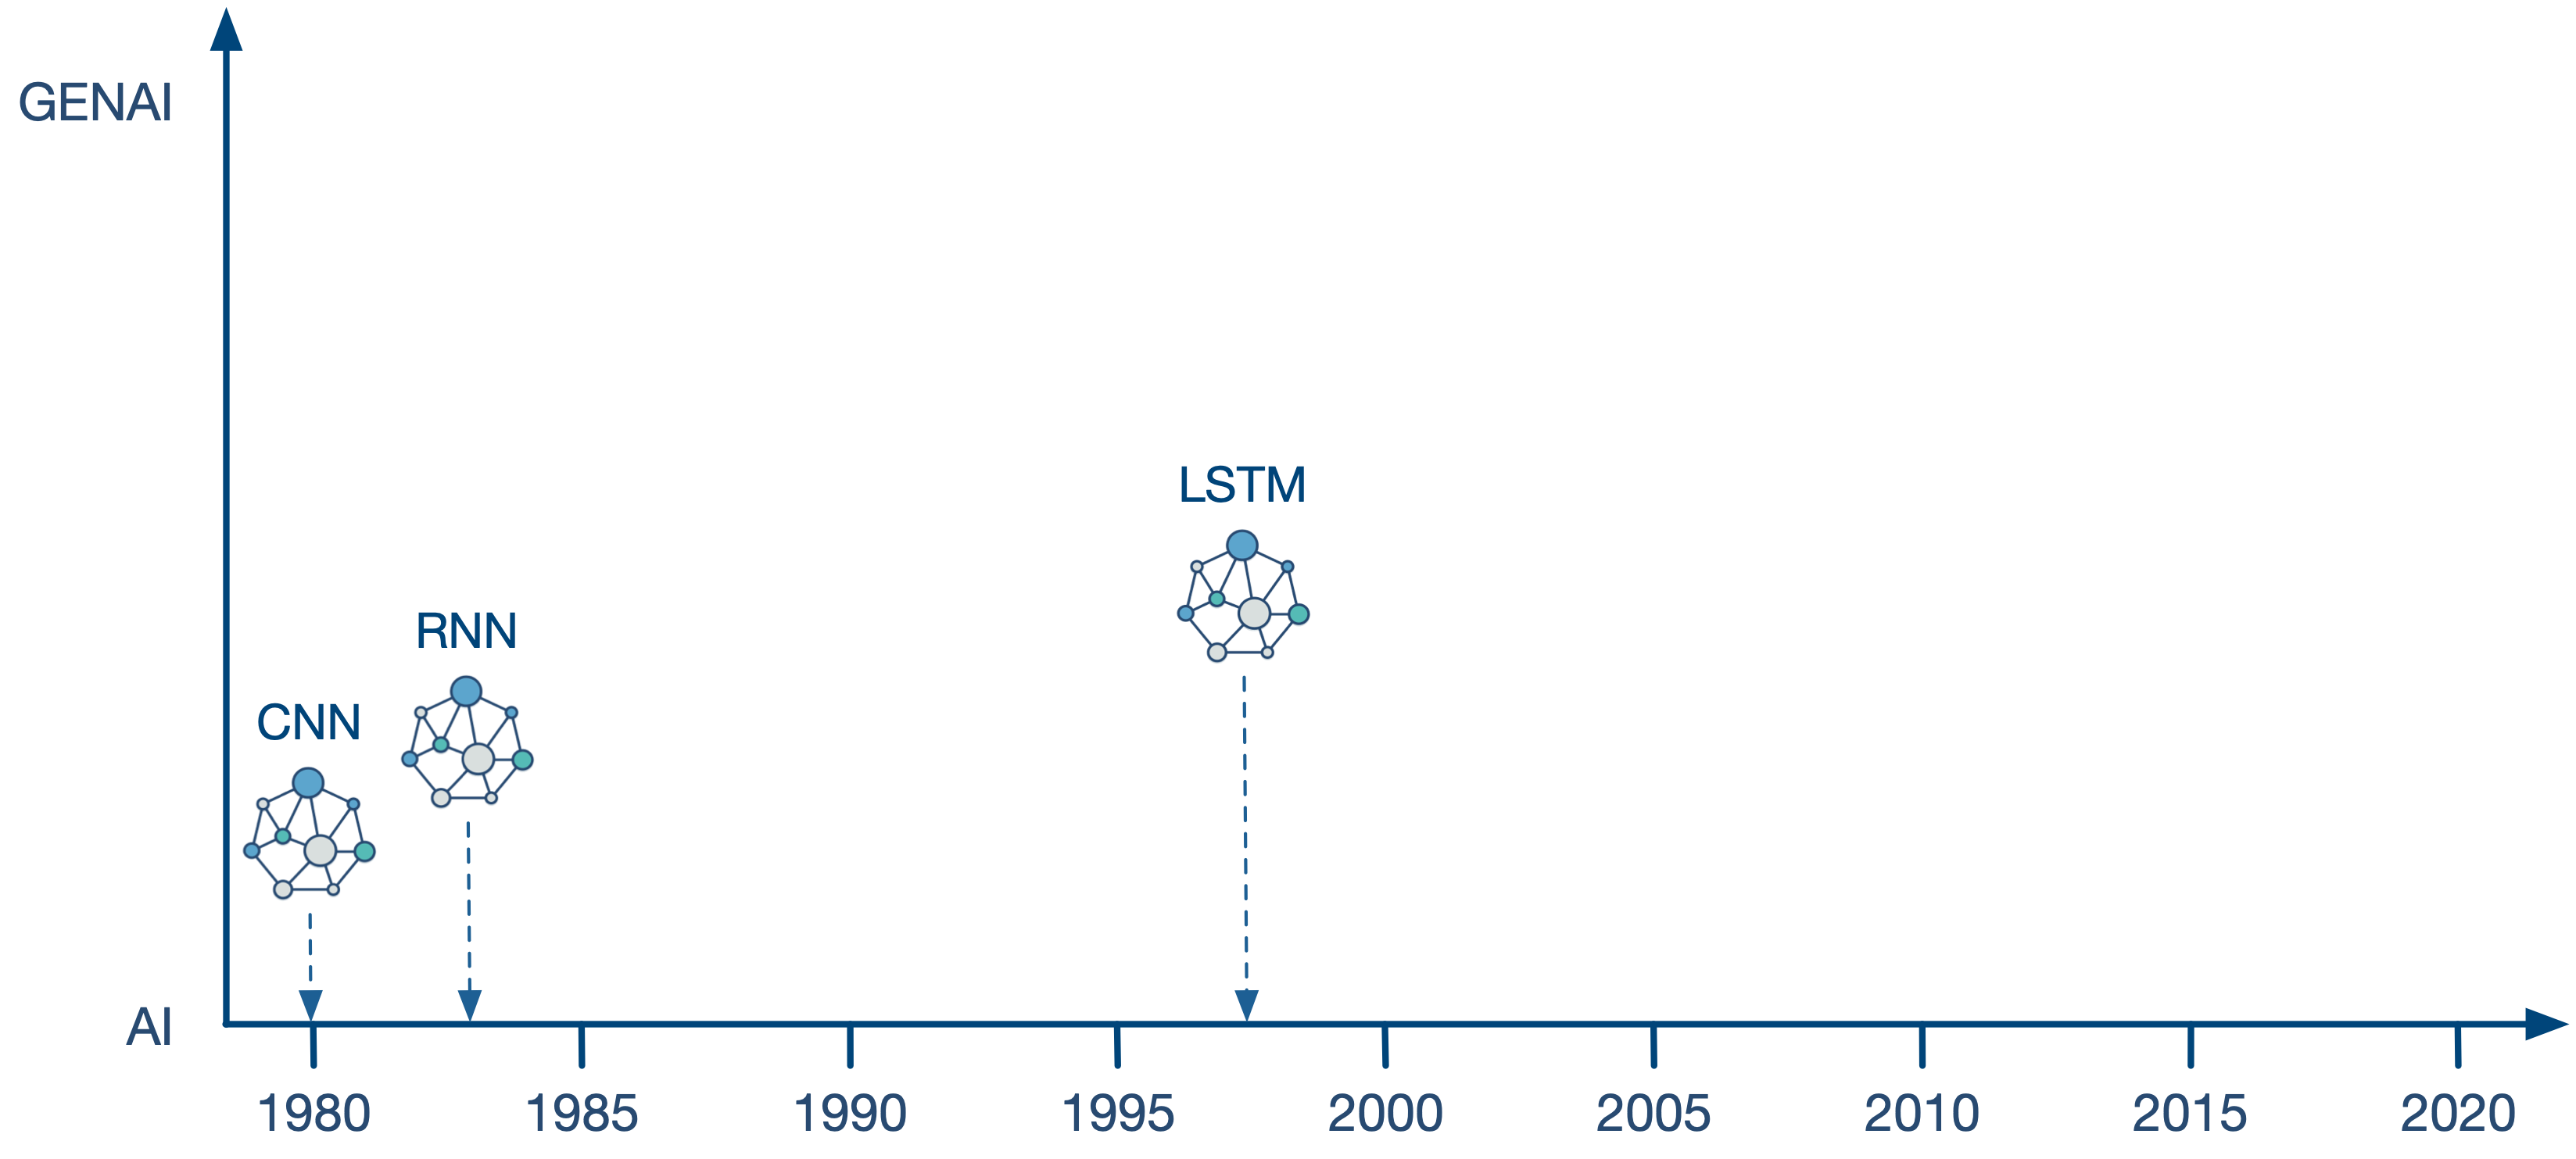
\includegraphics[width=\textwidth]{AI-GENAI-LSTM.png}
		\end{minipage}
	\end{figure}
}
	\only<5>{
	\begin{figure}[ht]
		\begin{minipage}[b]{0.95\linewidth}
			\centering
			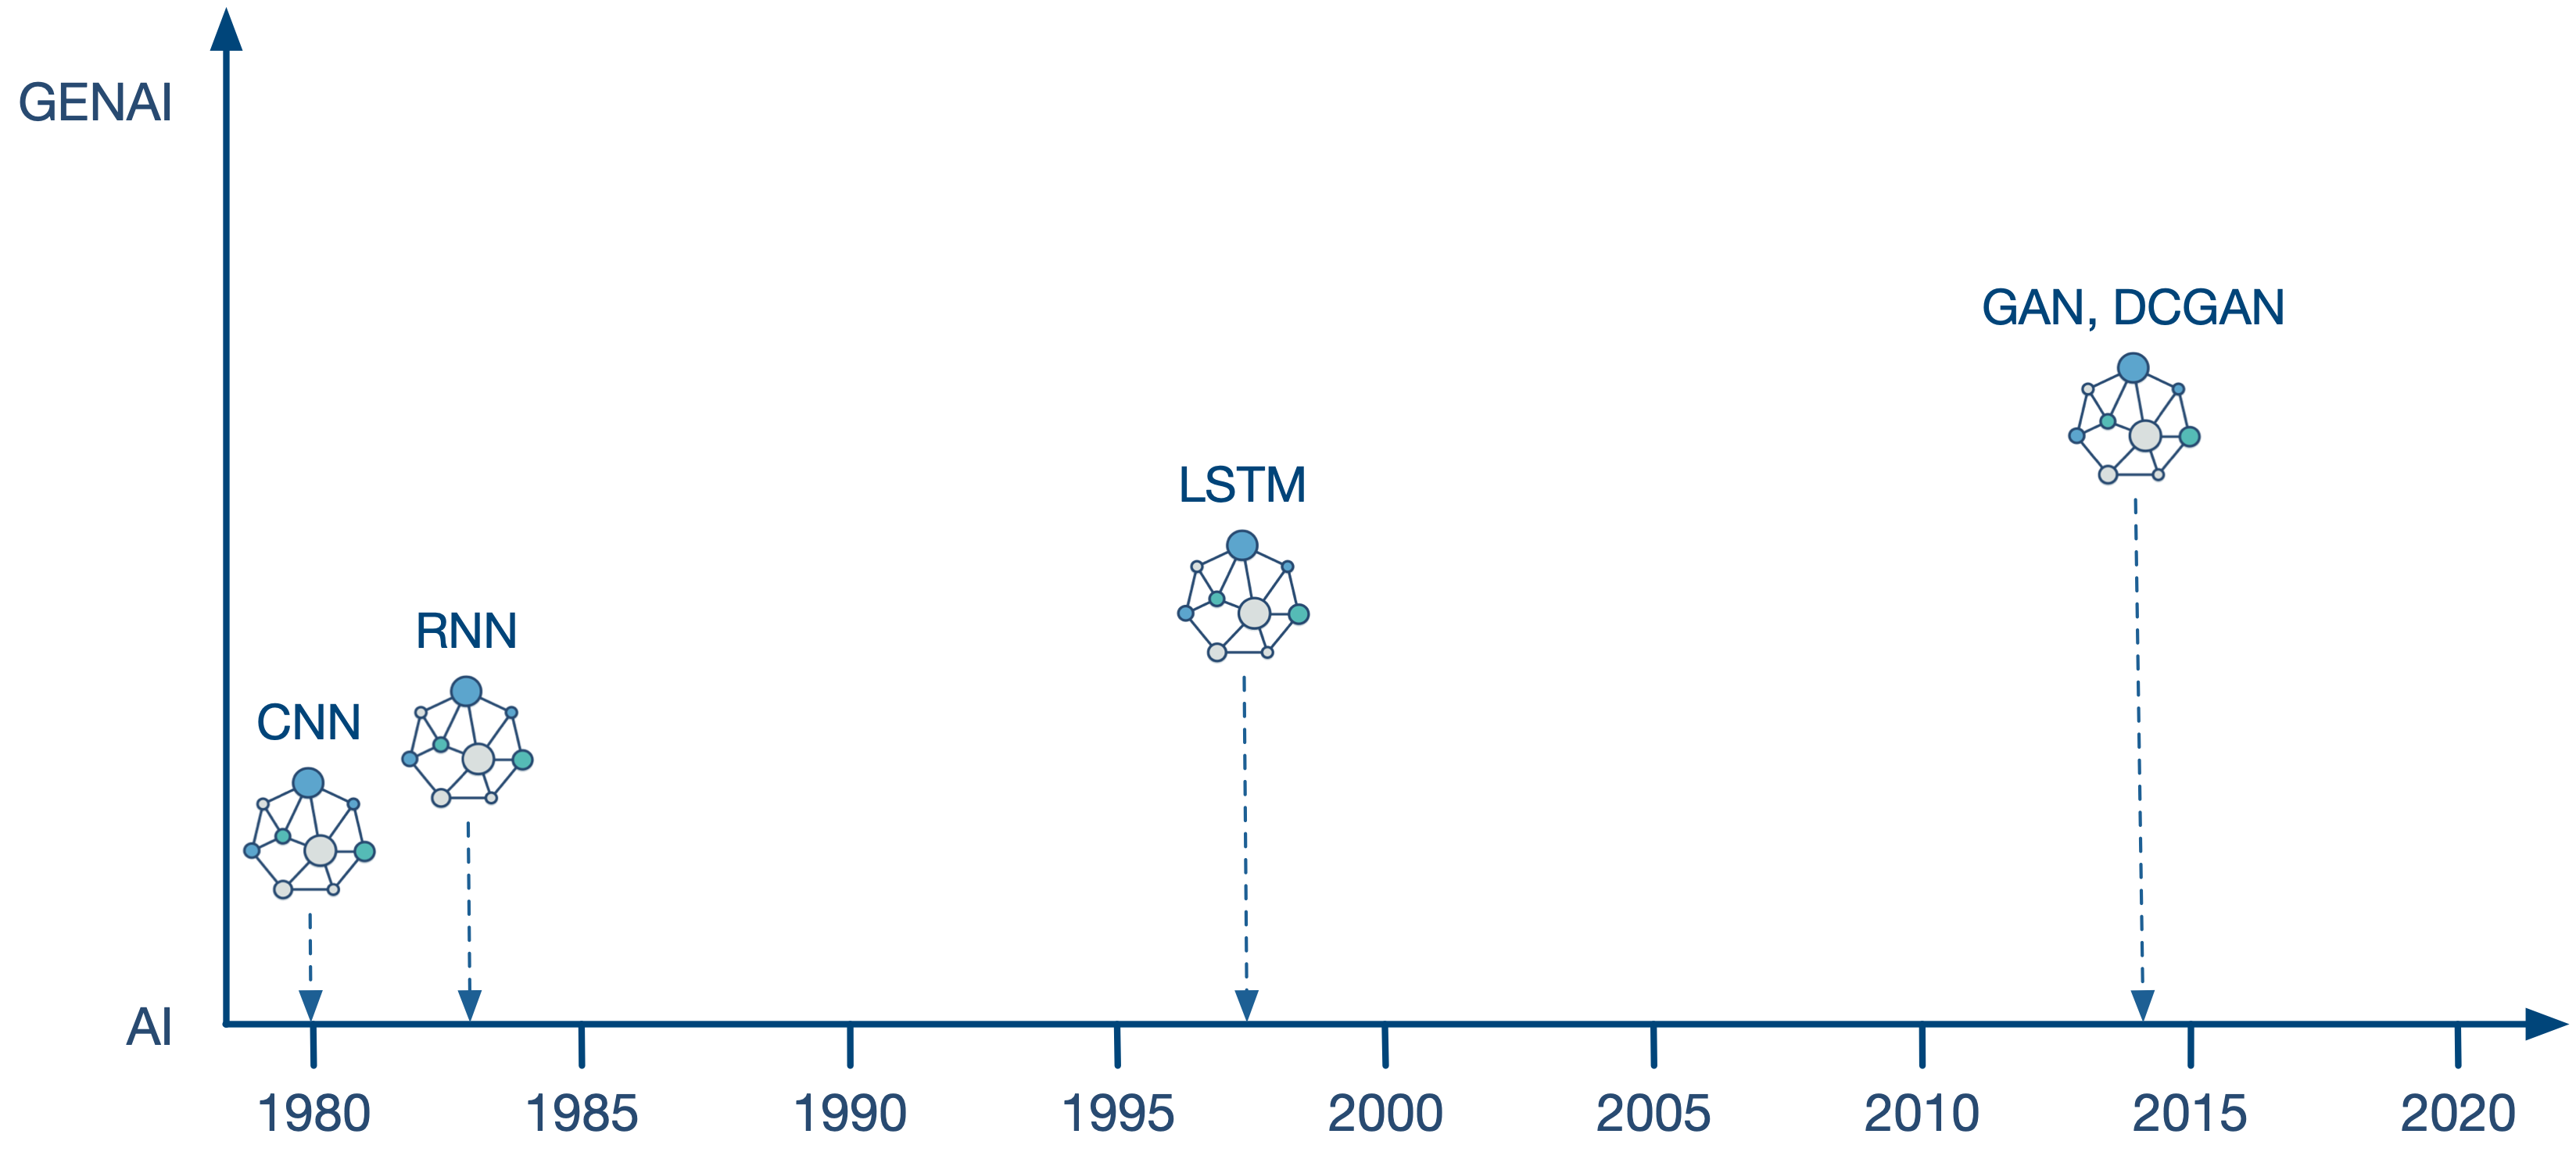
\includegraphics[width=\textwidth]{AI-GENAI-GAN.png}
		\end{minipage}
	\end{figure}
}
	\only<6>{
	\begin{figure}[ht]
		\begin{minipage}[b]{0.95\linewidth}
			\centering
			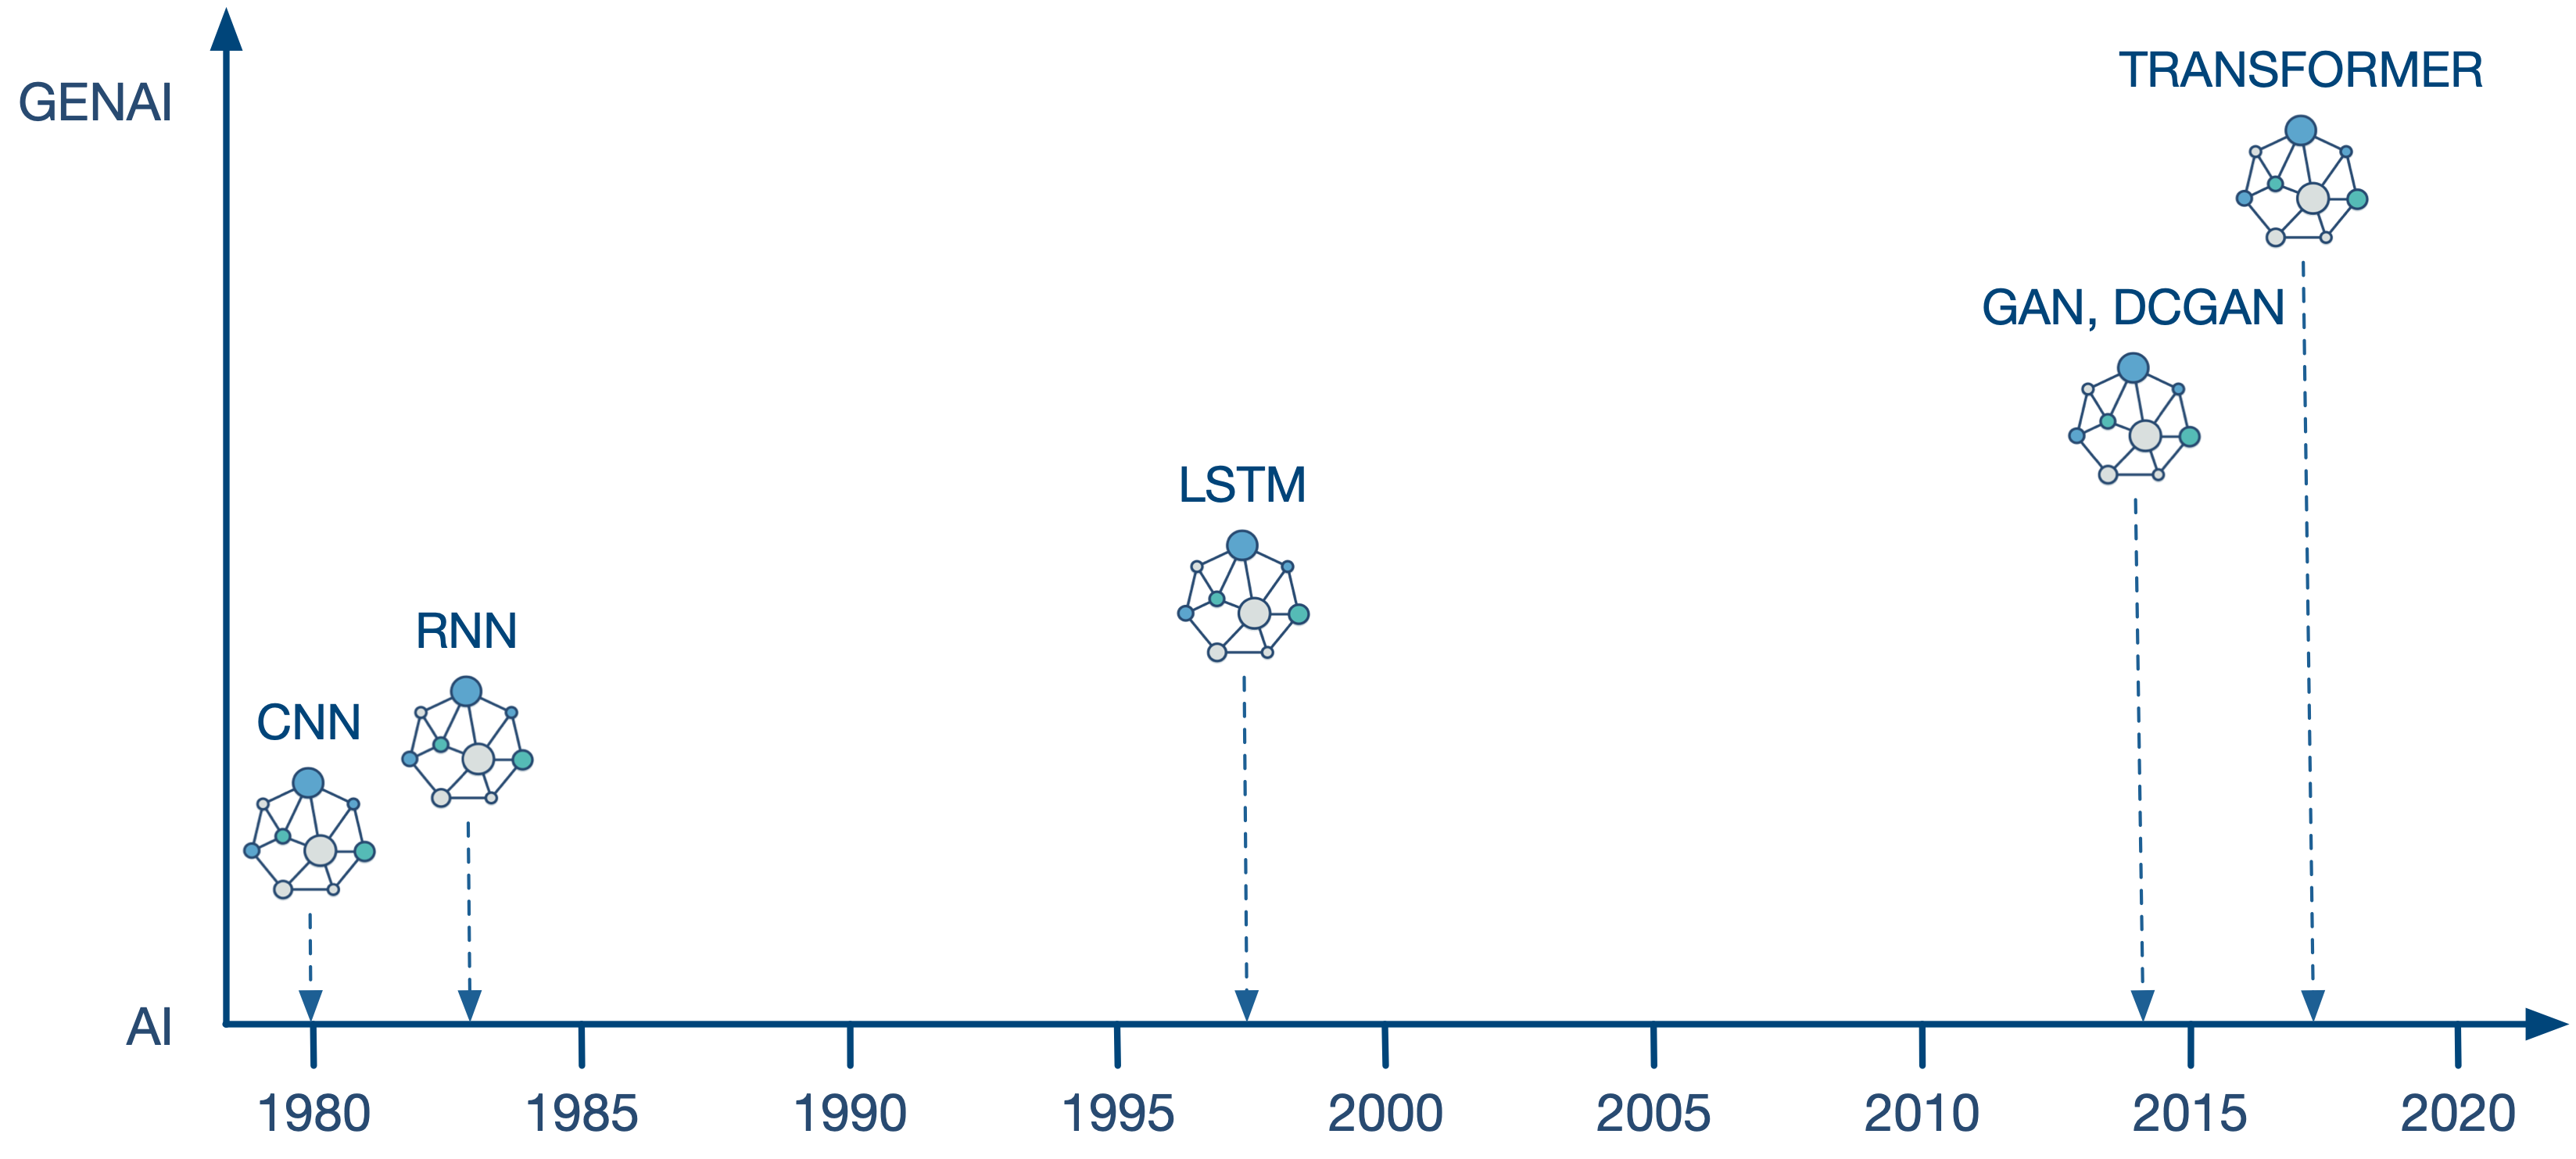
\includegraphics[width=\textwidth]{AI-GENAI-TRANS.png}
		\end{minipage}
	\end{figure}
}
}
\end{frame}
%
\begin{frame}[t] \frametitle{Architetture principali}
\framesubtitle{Recurrent Neural Network (RNN) - 1982}
{\scriptsize
\onslide<1->
	\begin{minipage}[t]{\textwidth}
		\begin{figure}
		    \centering
		    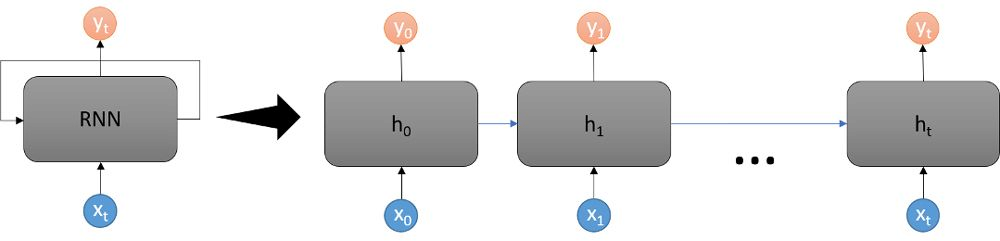
\includegraphics[width=.7\textwidth]{RNN.png}
            {\tiny\\Architettura RNN\\\textit{\textcopyright MathWorks}}
	    \end{figure}
        \begin{center}
            \vspace*{-.3cm}
            \href{https://cdn-images-1.medium.com/max/800/1*b4w12Ekzp_Vf6l0ntA0zWw.gif}{\faExternalLinkSquare\ ``Srotolamento'' unità RNN}
        \end{center}
    \end{minipage}
	\begin{minipage}[t]{\textwidth}
        \vspace*{.3cm}
		\begin{itemize}[leftmargin=10pt,align=right]
			\item[\alert{\faArrowCircleRight}] Ottimizzate per \emph{task} su dati ordinati/sequenziali
 		    \begin{itemize}[leftmargin=10pt,align=right] 
			    \item[\alert{\faArrowCircleRight}] Predizione di serie temporali, NLP, \emph{speech recognition}, \emph{video processing}
            \end{itemize}             
			\onslide<2->
			\item[\alert{\faArrowCircleRight}] Tiene traccia degli \emph{input} precedenti per influenzare l'\emph{input} e l'\emph{output} attuali
			\onslide<3->
			\item[\alert{\faArrowCircleRight}] Scardinano il principio di indipendenza tra \emph{layer}
			\onslide<4->
			\item[\alert{\faArrowCircleRight}] Condividono parametri a livello di \emph{layer} (come CNN)
			\begin{itemize}[leftmargin=10pt,align=right]
				\onslide<5->\item[\alert{\faArrowCircleRight}] \alert{Pro:} potenziale abbattimento dei tempi di addestramento/grandezza del modello addestrato
				\onslide<6->\item[\alert{\faArrowCircleRight}] \alert{Contro:} algoritmo di \emph{backpropagation} specifico, nel tempo (BPTT)
				\begin{itemize}[leftmargin=10pt,align=right]
					\item[\alert{\faArrowCircleRight}] Errore deve essere inteso come la somma degli errori fatti fino a quel momento
					\onslide<7->\item[\alert{\faArrowCircleRight}] \alert{Gradiente fantasma:} possibilità che addestramento smetta di imparare
					\onslide<8->\item[\alert{\faArrowCircleRight}] \alert{Gradiente che esplode:} possibilità di creare modelli instabili, con pesi troppo grandi
				\end{itemize}
			\end{itemize}
		\end{itemize}
	\end{minipage}
}
\end{frame}
%
\begin{frame}[t] \frametitle{Architetture principali}
\framesubtitle{Long Short-Term Memory (LSTM) - 1997}
{\scriptsize
\vspace*{-.5cm}
\onslide<1->
	\begin{minipage}[t]{\textwidth}
		\begin{figure}
			\centering
			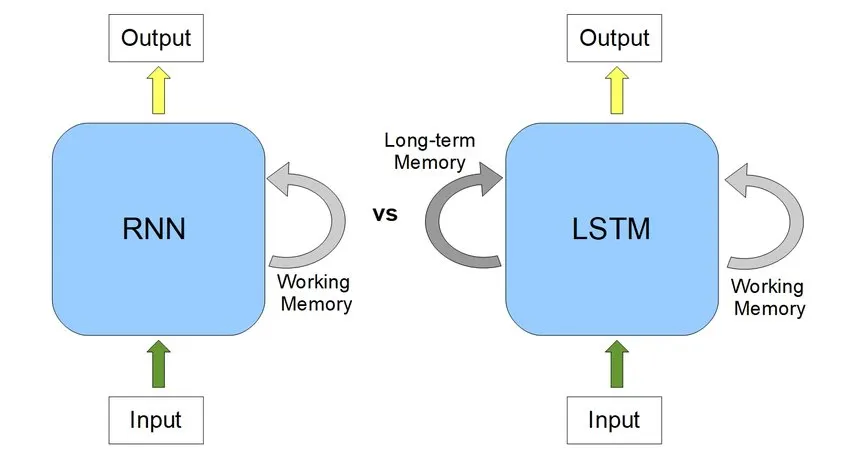
\includegraphics[width=.5\textwidth]{RNN-vs-LSTM-no-bg.png}
			\\RNN vs LSTM\textsuperscript{\textcopyright}Fiverr
		\end{figure}
	\end{minipage}
	\\\vspace*{.3cm}
	\begin{minipage}[t]{\textwidth}
	\begin{itemize}[leftmargin=10pt,align=right]
		\onslide<1->\item[\alert{\faArrowCircleRight}] Varianti più avanzate delle RNN
		\begin{itemize}[leftmargin=10pt,align=right]
			\item[\alert{\faArrowCircleRight}] La memoria a breve termine può durare migliaia di passaggi (da cui il termine \emph{long})
			\onslide<2->\item[\alert{\faArrowCircleRight}] Gli \emph{hidden layer} usano unità a tre porte (\emph{in}/\emph{out}/\emph{forget})
			\onslide<3->\item[\alert{\faArrowCircleRight}] Il \emph{forget} permette di tralasciare elementi reputati non più importanti per la decisione dell'\emph{output} corrente
		\end{itemize}
	\end{itemize}
	\end{minipage}
}
\end{frame}
%
\begin{frame}[t] \frametitle{Architetture principali}
\framesubtitle{RNN vs LSTM}
{\scriptsize
\onslide<1->
	\begin{minipage}[t]{\textwidth}
		\begin{figure}
			\centering
			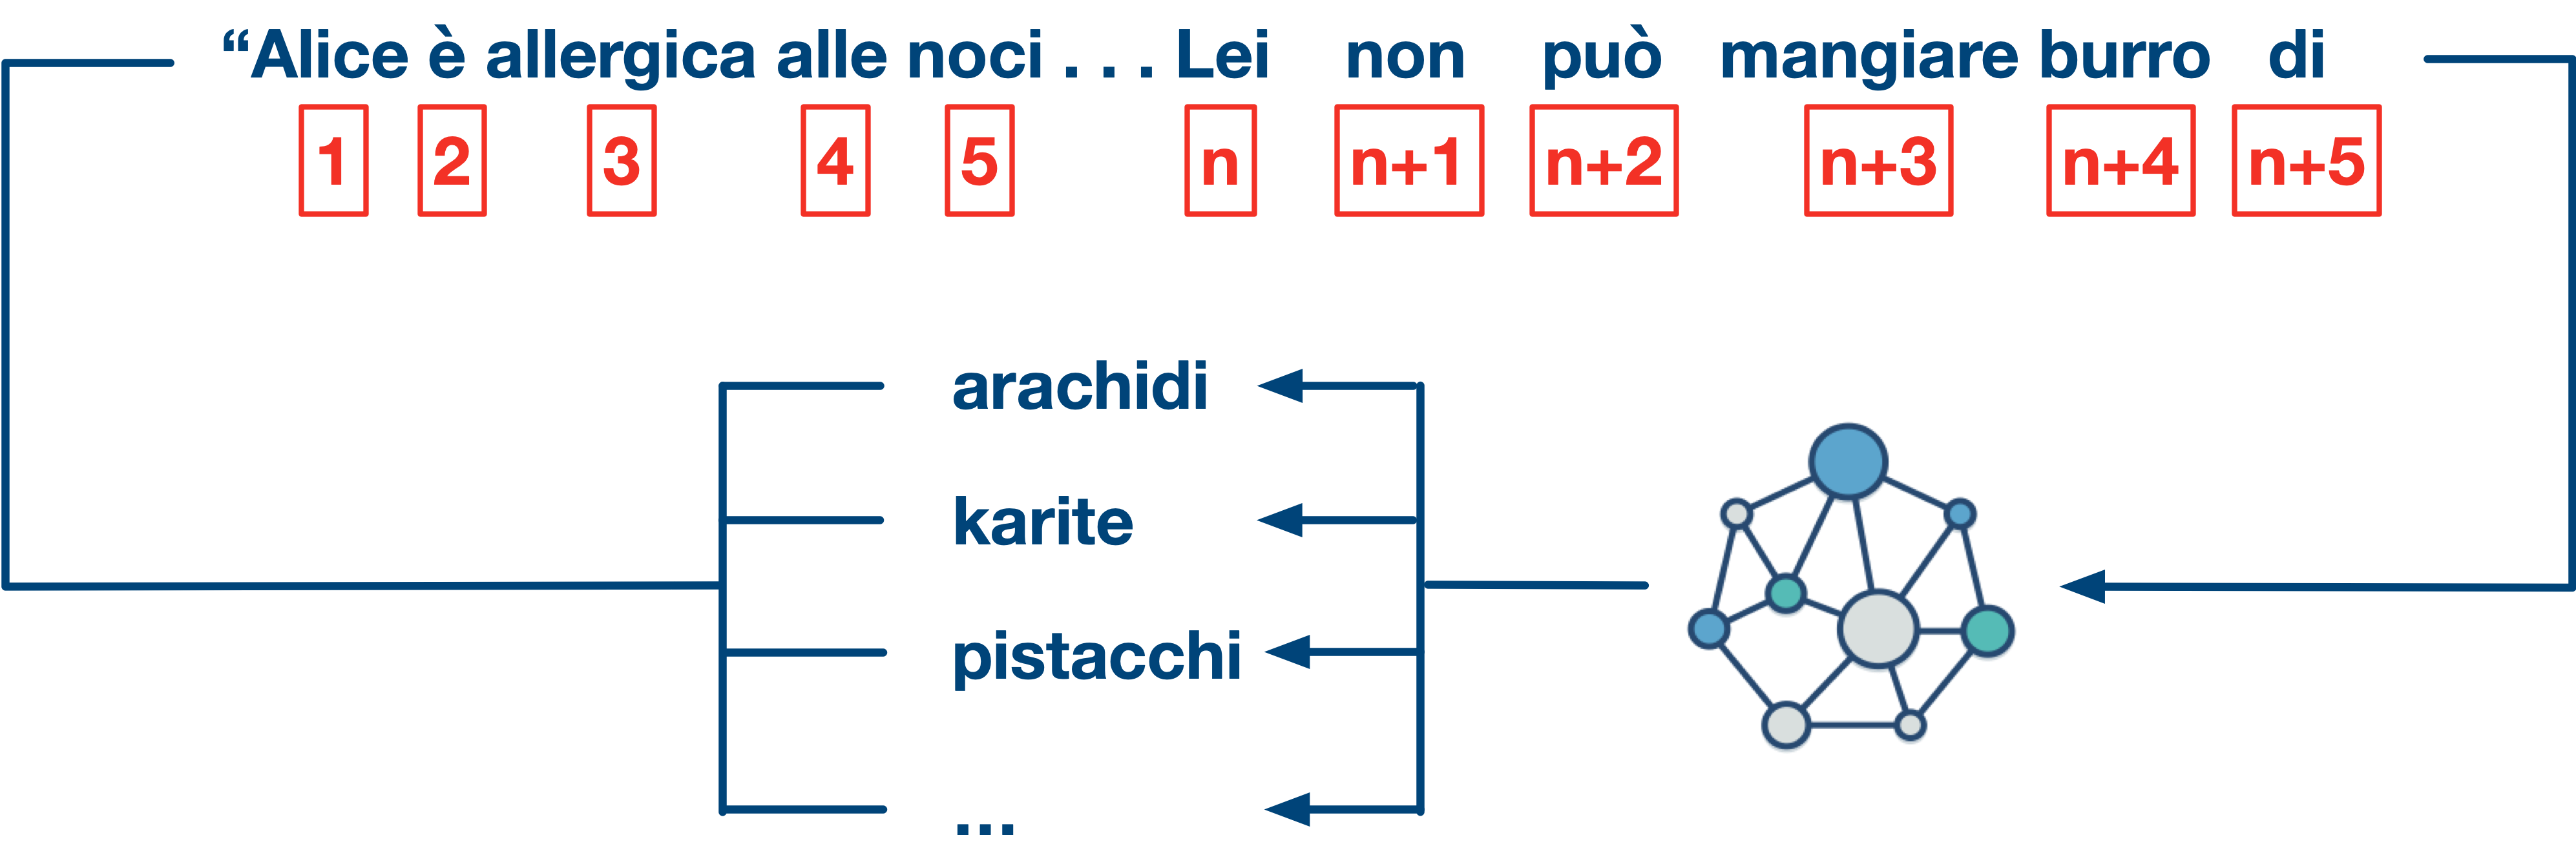
\includegraphics[width=.7\textwidth]{RNN-vs-LSTM-example.png}
			\\RNN vs LSTM
		\end{figure}
	\end{minipage}
	\\\vspace*{.3cm}
	\begin{minipage}[t]{\textwidth}
		\begin{itemize}[leftmargin=10pt,align=right]
			\onslide<2->\item[\alert{\faArrowCircleRight}] Cosa succede se $n \approx 5$?
			\begin{itemize}[leftmargin=10pt,align=right]
				\onslide<3->\item[\alert{\faArrowCircleRight}] CNN ed LSTM si comportano in maniera simile
			\end{itemize}
			\onslide<4->\item[\alert{\faArrowCircleRight}] Cosa succede se $n \gg 5$?
			\begin{itemize}[leftmargin=10pt,align=right]
				\onslide<5->\item[\alert{\faArrowCircleRight}] LSTM probabilmente avrà probabilità alte in corrispondenza della frutta secca$\ldots$
				\onslide<6->\item[\alert{\faArrowCircleRight}] $\ldots$RNN assicurerebbe una crisi anafilattica ad Alice!
			\end{itemize}
		\end{itemize}
	\end{minipage}
}
\end{frame}
%
\begin{frame}[t] \frametitle{Architetture principali}
\framesubtitle{Generative Adversarial Network (GAN)}
{\scriptsize
\onslide<1->
	\begin{minipage}[t]{\textwidth}
		\begin{figure}
			\centering
			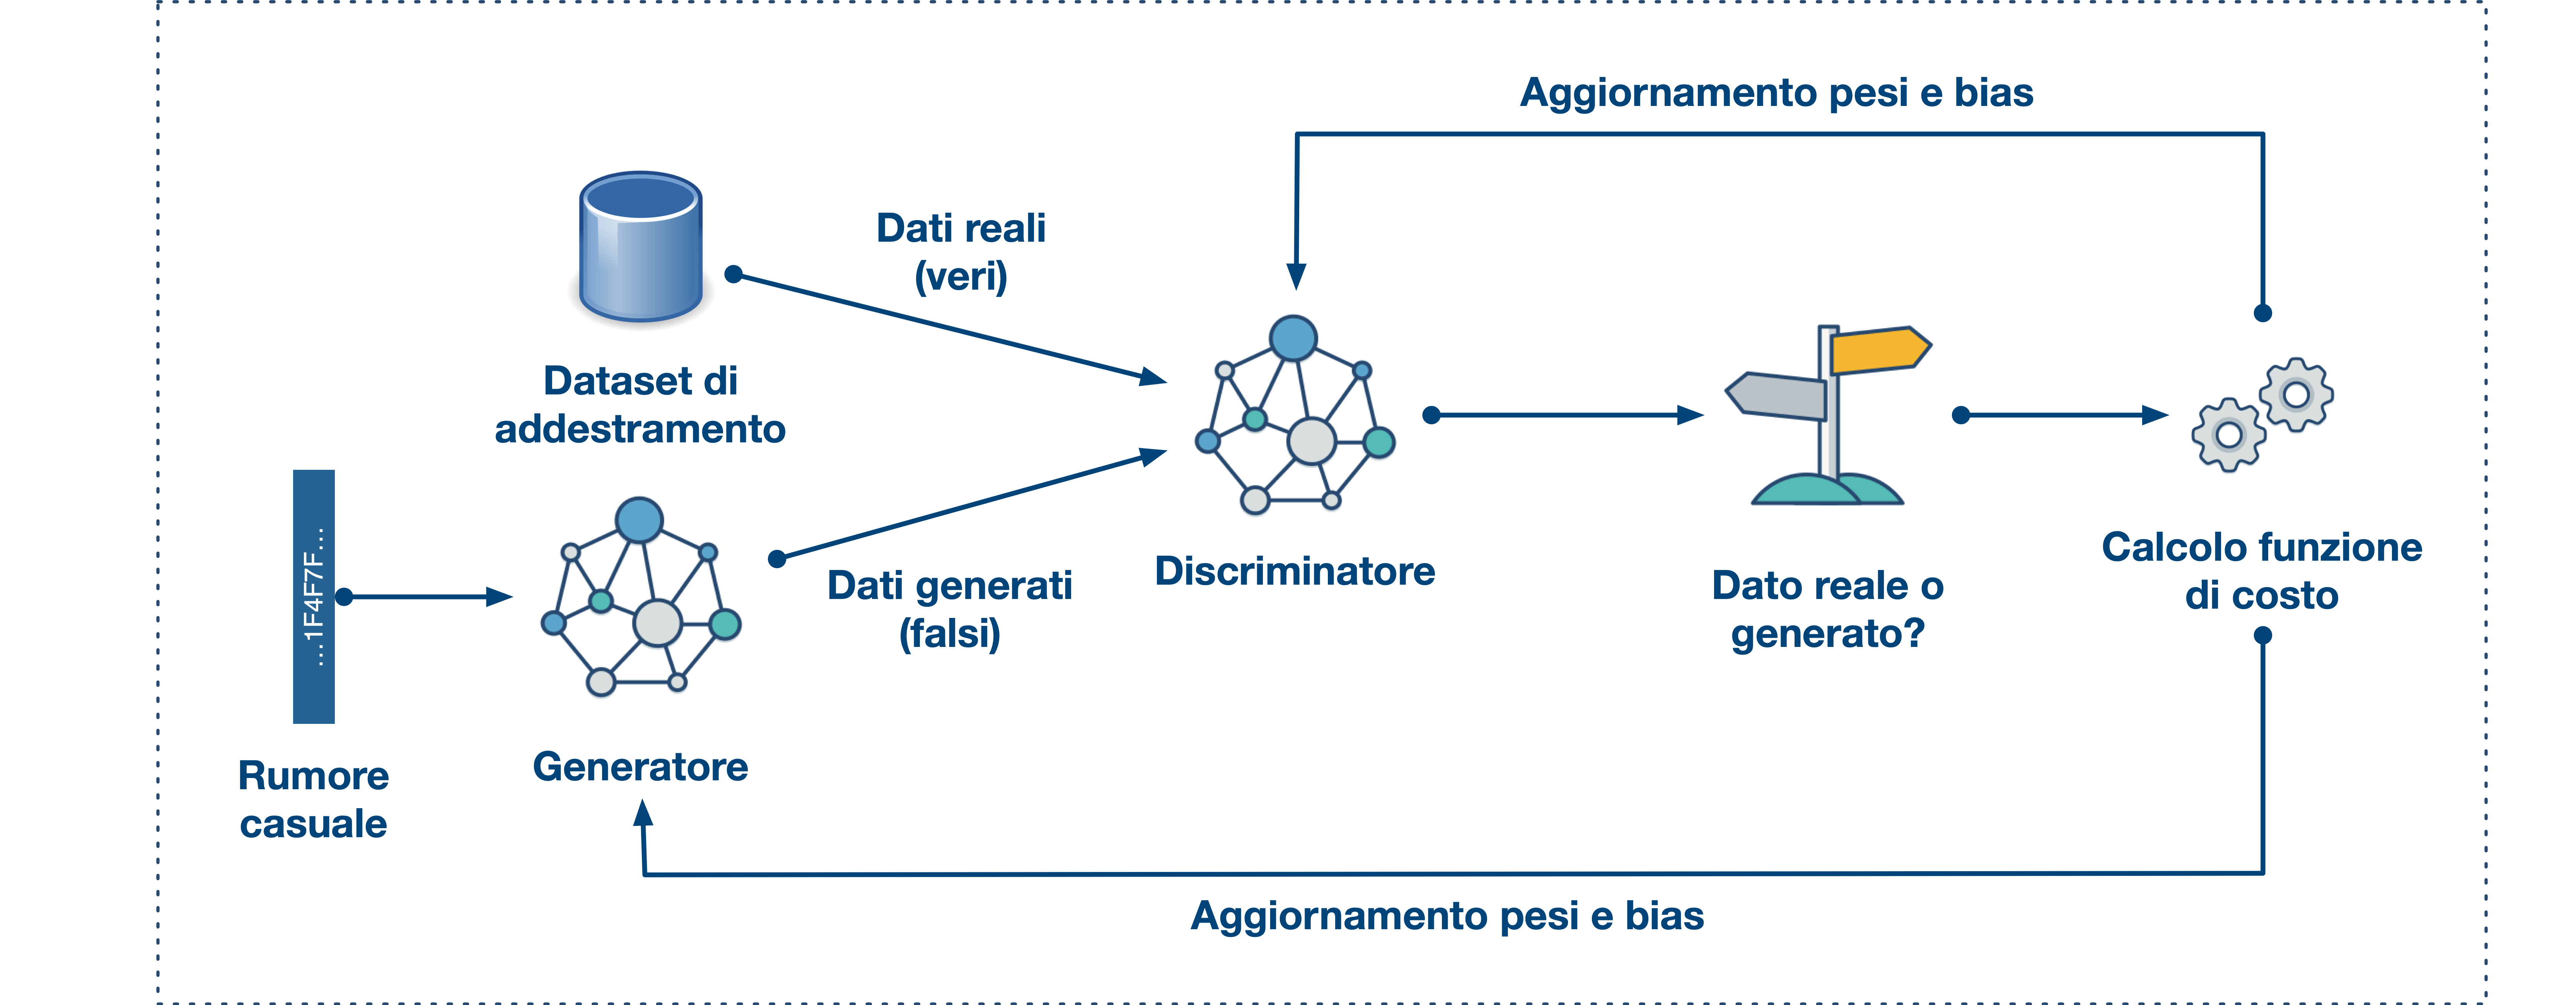
\includegraphics[width=.5\textwidth]{GAN.png}
			\\Architettura GAN
		\end{figure}
	\end{minipage}
	\\\vspace*{.3cm}
	\begin{minipage}[t]{\textwidth}
		\begin{itemize}[leftmargin=10pt,align=right]
			\item[\alert{\faArrowCircleRight}] Nato come concetto algoritmico nel 2014 e reso teoricamente più robusto nel 2016 (\emph{\alert{D}eep \alert{C}onvolutional \alert{GAN}} -- \alert{DCGAN})
			\onslide<2->\item[\alert{\faArrowCircleRight}] Prima rivoluzione nel modo in cui si creano contenuti artificiali
			\onslide<3->\item[\alert{\faArrowCircleRight}] Due reti neurali che competono
			\begin{itemize}[leftmargin=10pt,align=right]
				\onslide<4->\item[\alert{\faArrowCircleRight}] \alert{Generatore}
				\begin{itemize}[leftmargin=10pt,align=right]
					\item[\alert{\faArrowCircleRight}] \alert{Obiettivo:} migliorare la qualità dei contenuti che produce, ingannando il discriminatore
					\item[\alert{\faArrowCircleRight}] Crea un campione di dati
				\end{itemize}
				\onslide<5->\item[\alert{\faArrowCircleRight}] \alert{Discriminatore}
				\begin{itemize}[leftmargin=10pt,align=right]
					\item[\alert{\faArrowCircleRight}] \alert{Obiettivo:} migliorare l'abilità di discriminare dati reali da quelli prodotti
					\item[\alert{\faArrowCircleRight}] Decide se il campione è generato oppure preso dal campione reale (classificazione binaria)
				\end{itemize}
			\end{itemize}
		\end{itemize}
	\end{minipage}
}
\end{frame}
%
\begin{frame}[t] \frametitle{Architetture principali}
\framesubtitle{GAN - Addestramento}
{\scriptsize
\onslide<1->
	\begin{minipage}[t]{\textwidth}
		\begin{figure}
			\centering
			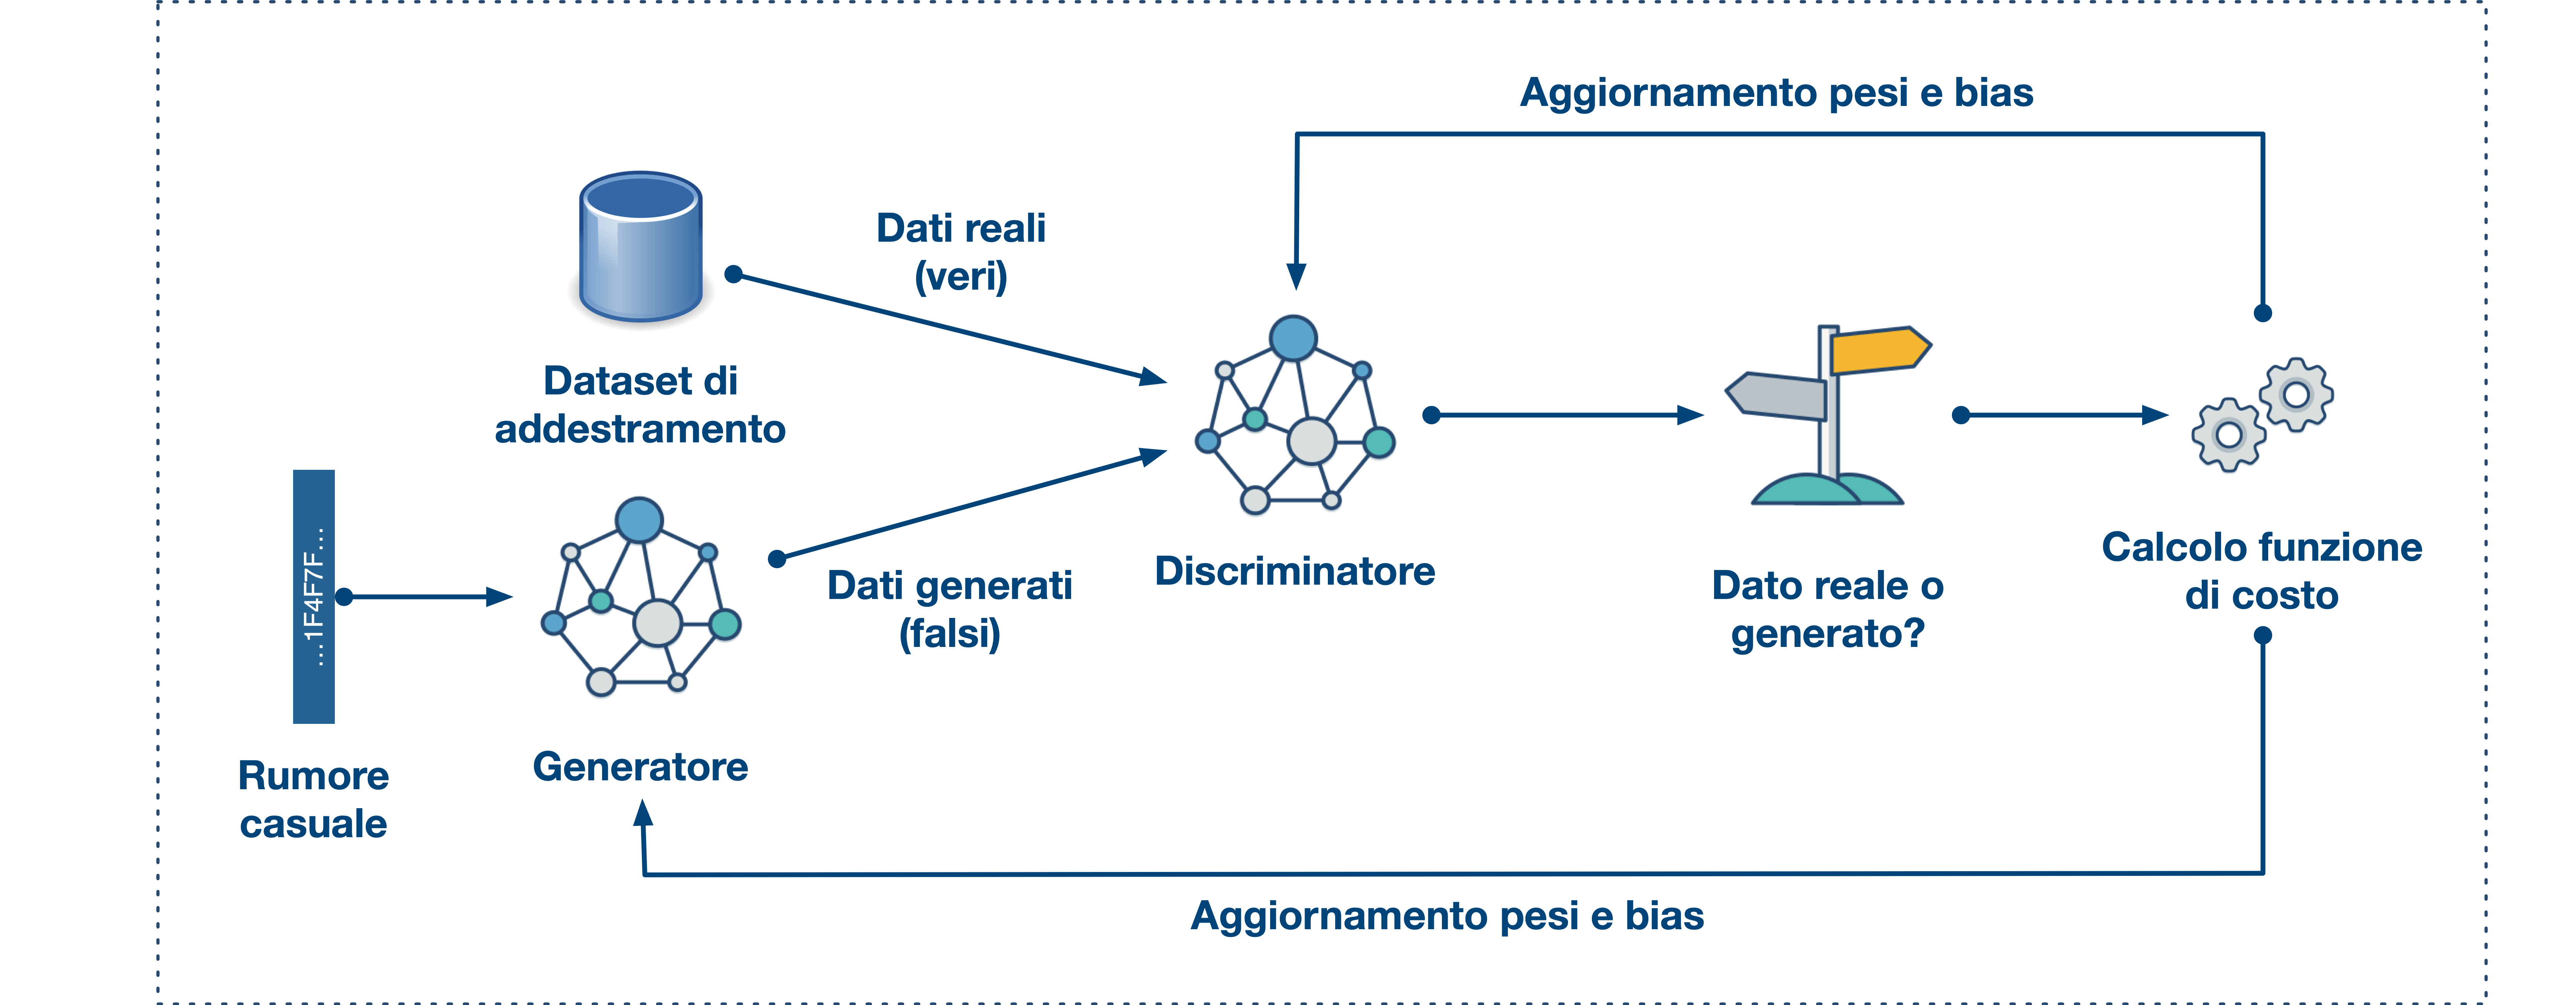
\includegraphics[width=.5\textwidth]{GAN.png}
			\\Architettura GAN
		\end{figure}
	\end{minipage}
	\\\vspace*{.3cm}
	\begin{minipage}[t]{\textwidth}
		\begin{enumerate}[leftmargin=10pt,align=right]
			\onslide<1->\item[\circled{alerted text.fg}{white}{1}] Addestrare il discriminatore sui dati reali (\emph{dataset} di addestramento)
			\onslide<2->\item[\circled{alerted text.fg}{white}{2}] Generare i dati falsi per il discriminatore
			\onslide<3->\item[\circled{alerted text.fg}{white}{3}] Addestrare il discriminatore sui dati falsi
			\onslide<4->\item[\circled{alerted text.fg}{white}{4}] Addestrare il generatore con l'\emph{output} del discriminatore
		\end{enumerate}
		\vspace*{.5cm}
		\begin{itemize}[leftmargin=10pt,align=right]
					\item[\alert{\faArrowCircleRight}] $\ldots$ giusto per farvi capire la complessità del processo$\ldots$
		\end{itemize}
	\end{minipage}
}
\end{frame}
%
\begin{frame}[t] \frametitle{GENAI}
\framesubtitle{Limitazioni e contro in NLP}
{\scriptsize
\only<1>{
	\begin{figure}[ht]
		\begin{minipage}[b]{0.95\linewidth}
			\centering
			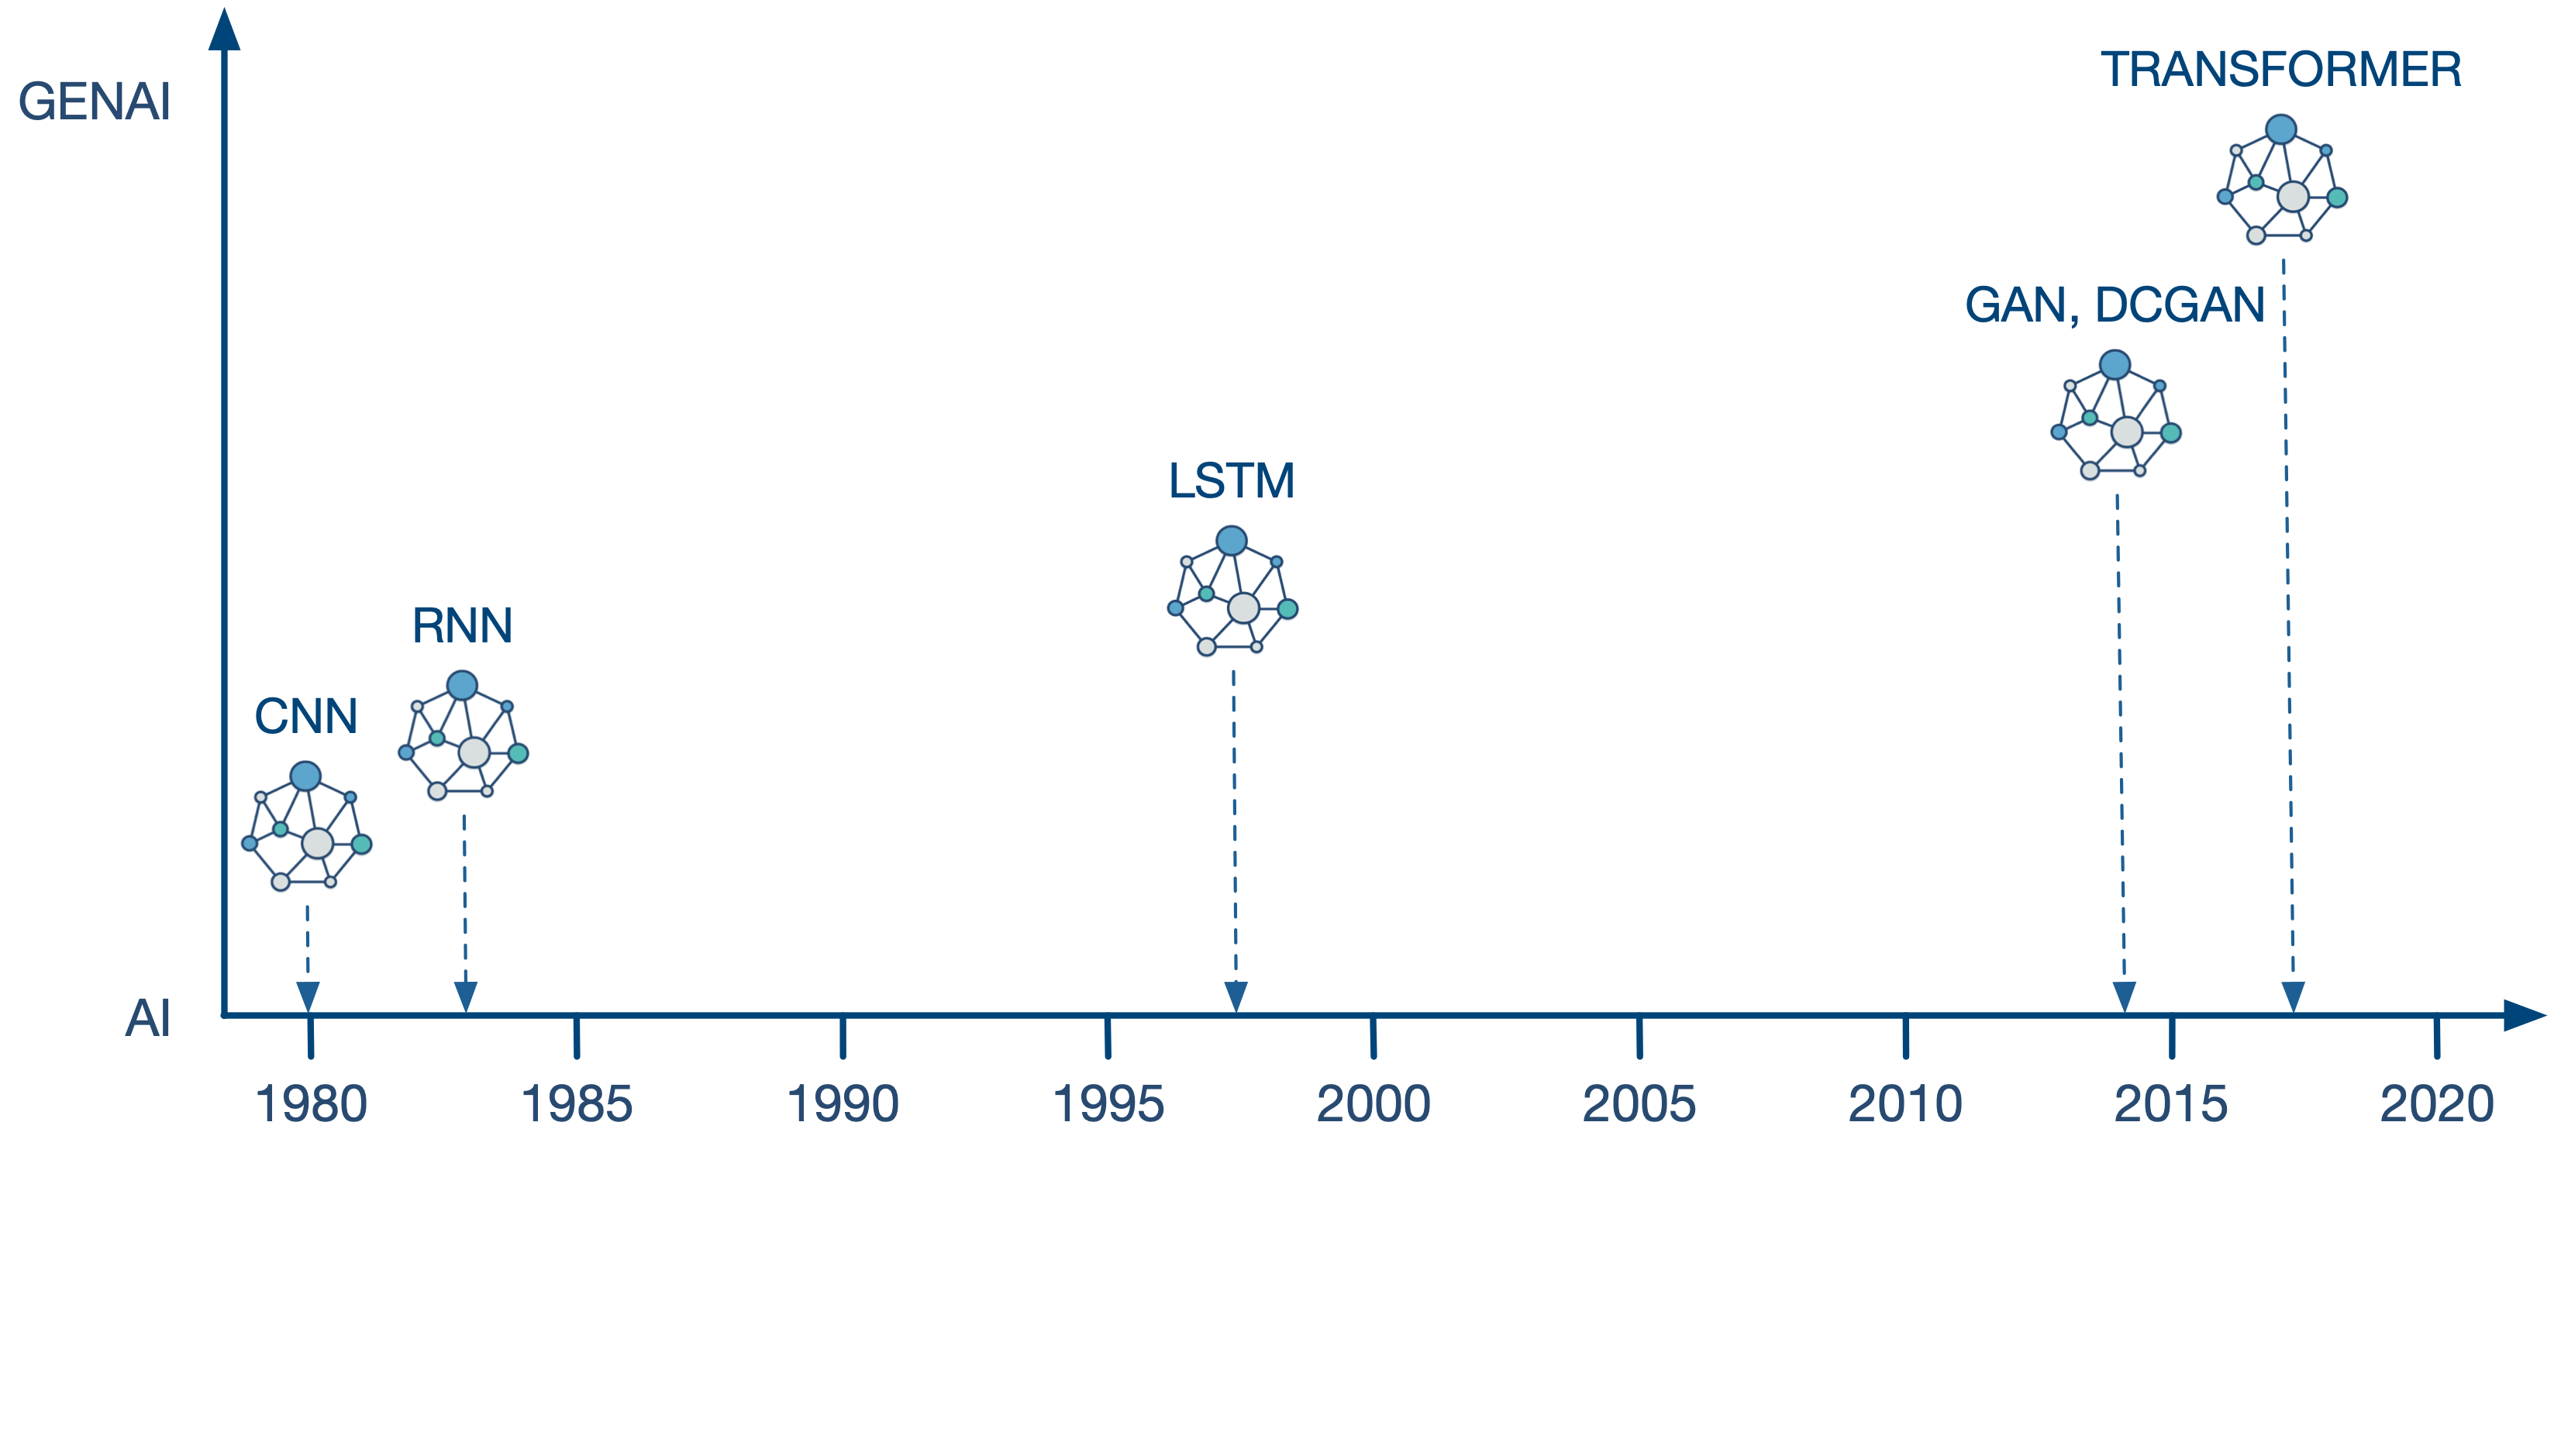
\includegraphics[width=\textwidth]{AI-GENAI-NLP-problems-0.png}
		\end{minipage}
	\end{figure}
}
	\only<2>{
	\begin{figure}[ht]
		\begin{minipage}[b]{0.95\linewidth}
			\centering
			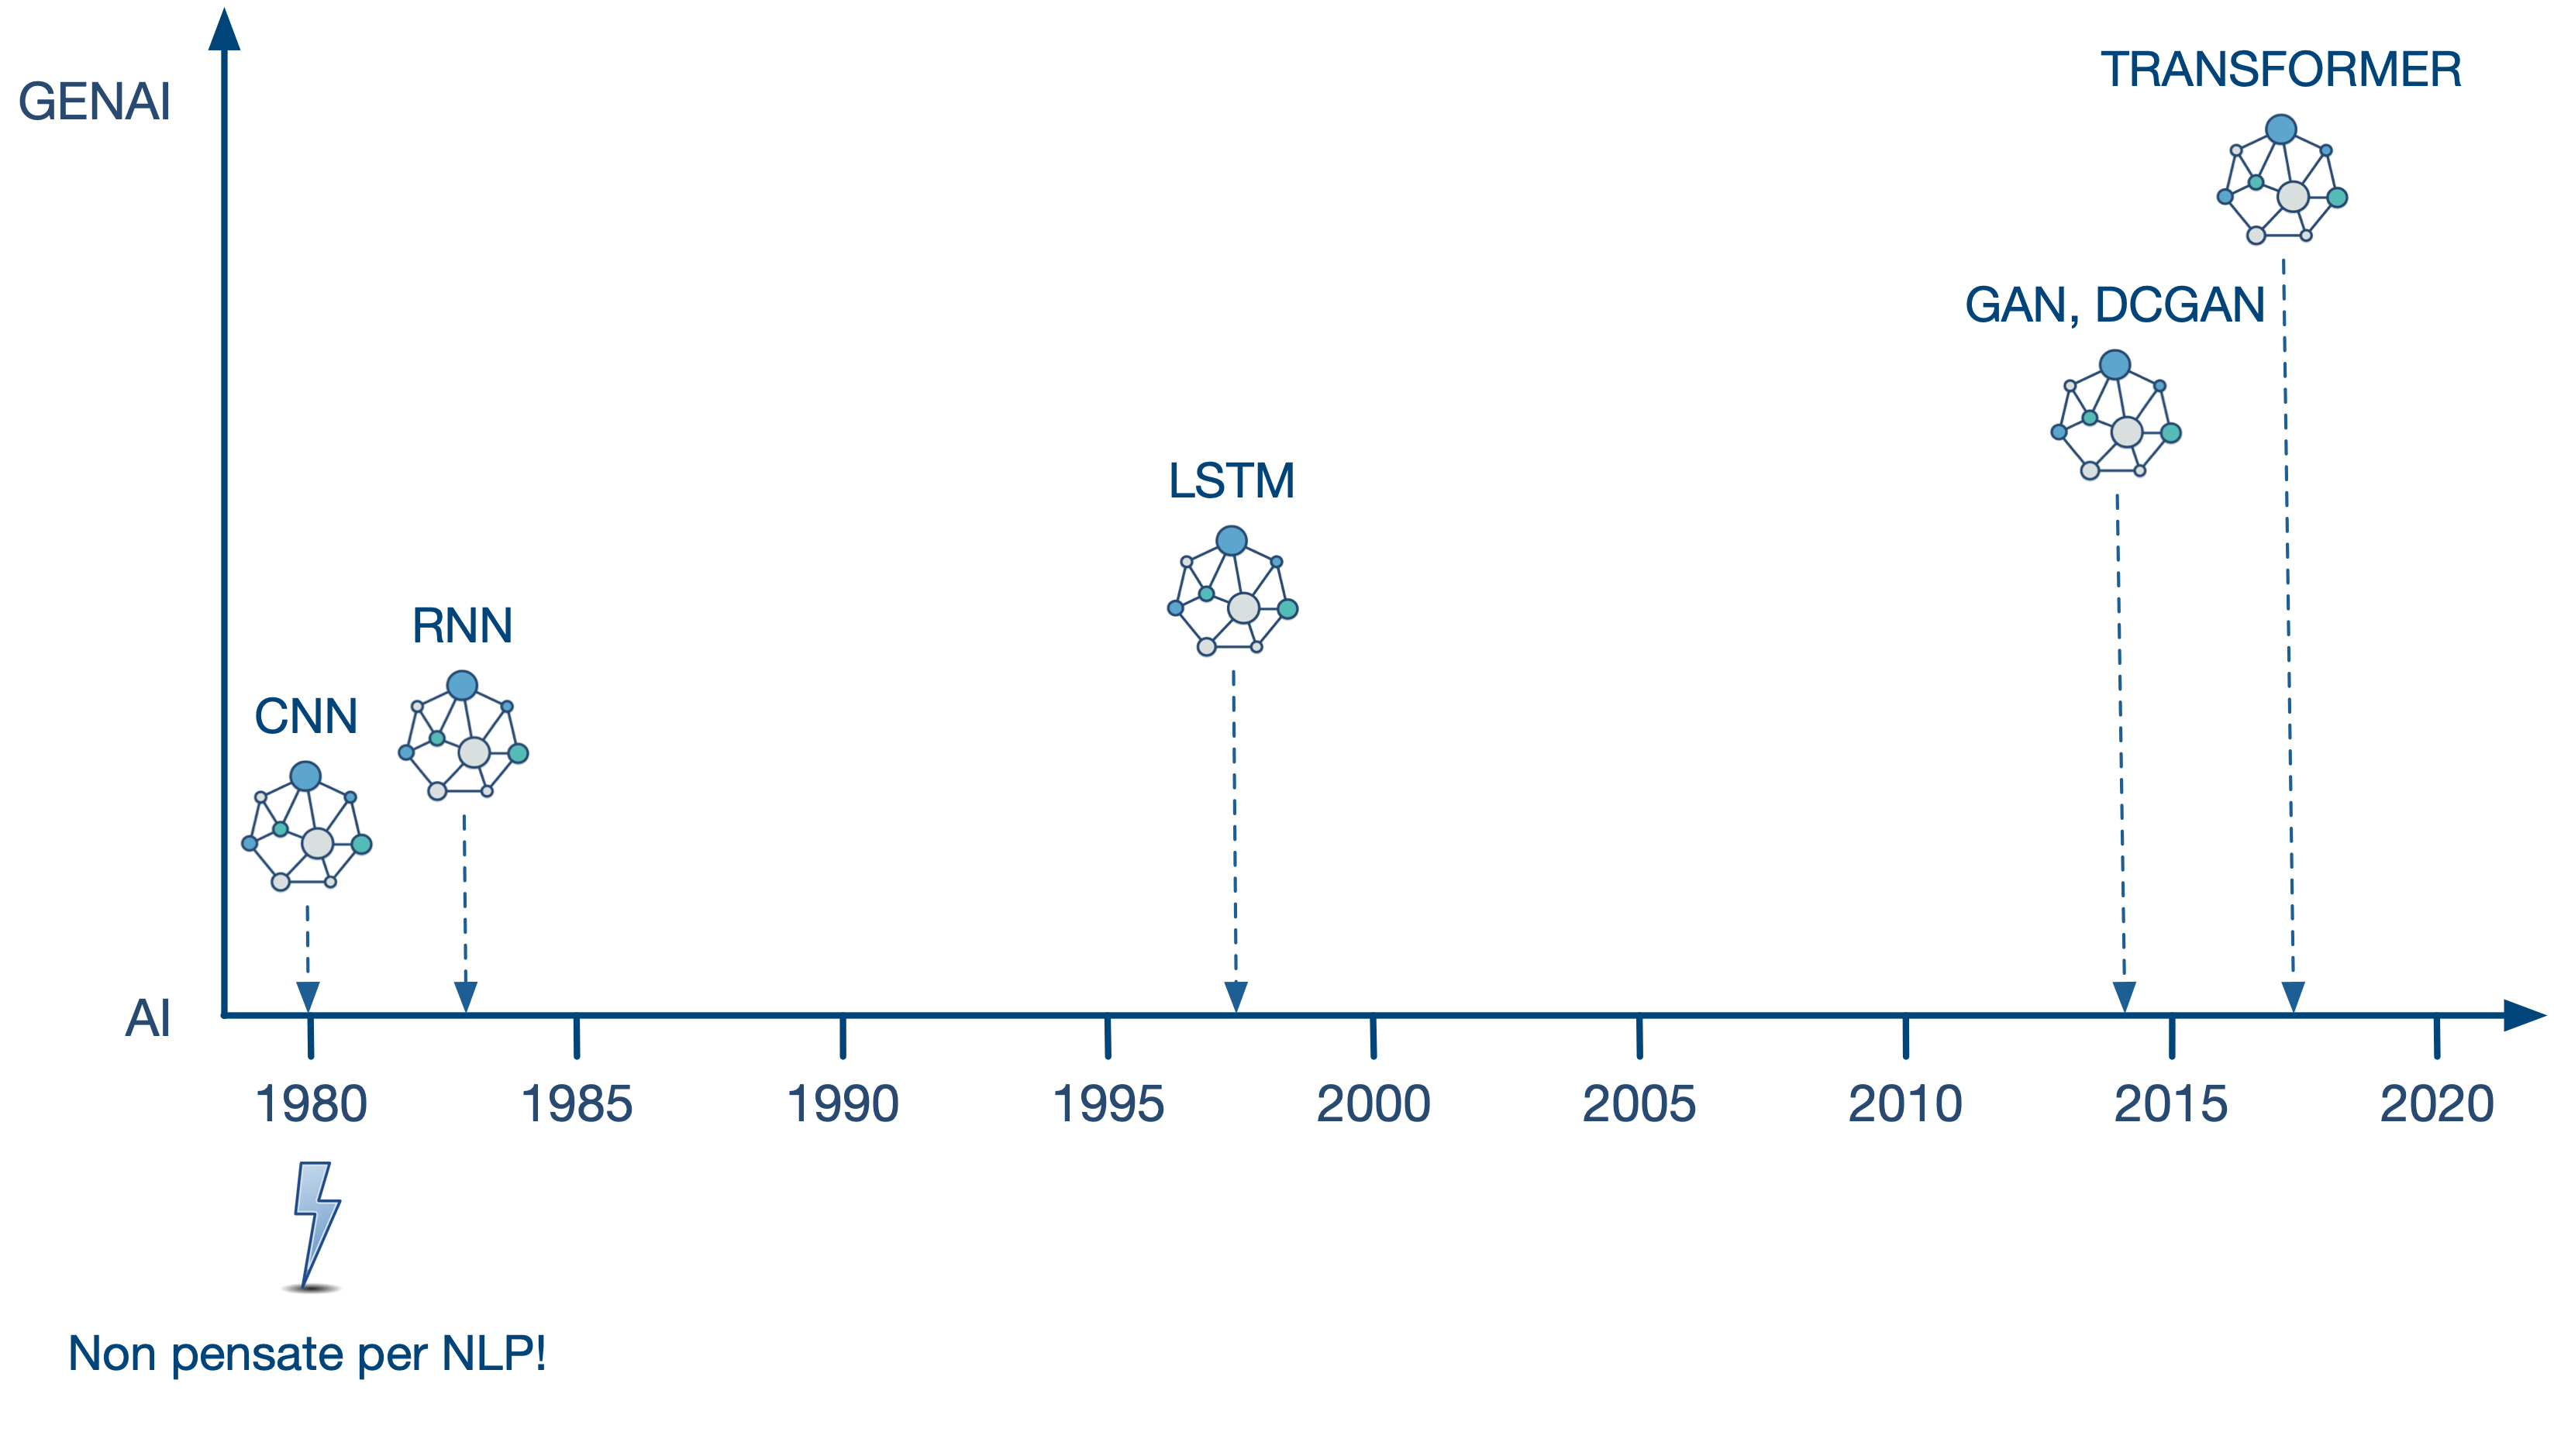
\includegraphics[width=\textwidth]{AI-GENAI-NLP-problems-1.png}
		\end{minipage}
	\end{figure}
}
	\only<3>{
	\begin{figure}[ht]
		\begin{minipage}[b]{0.95\linewidth}
			\centering
			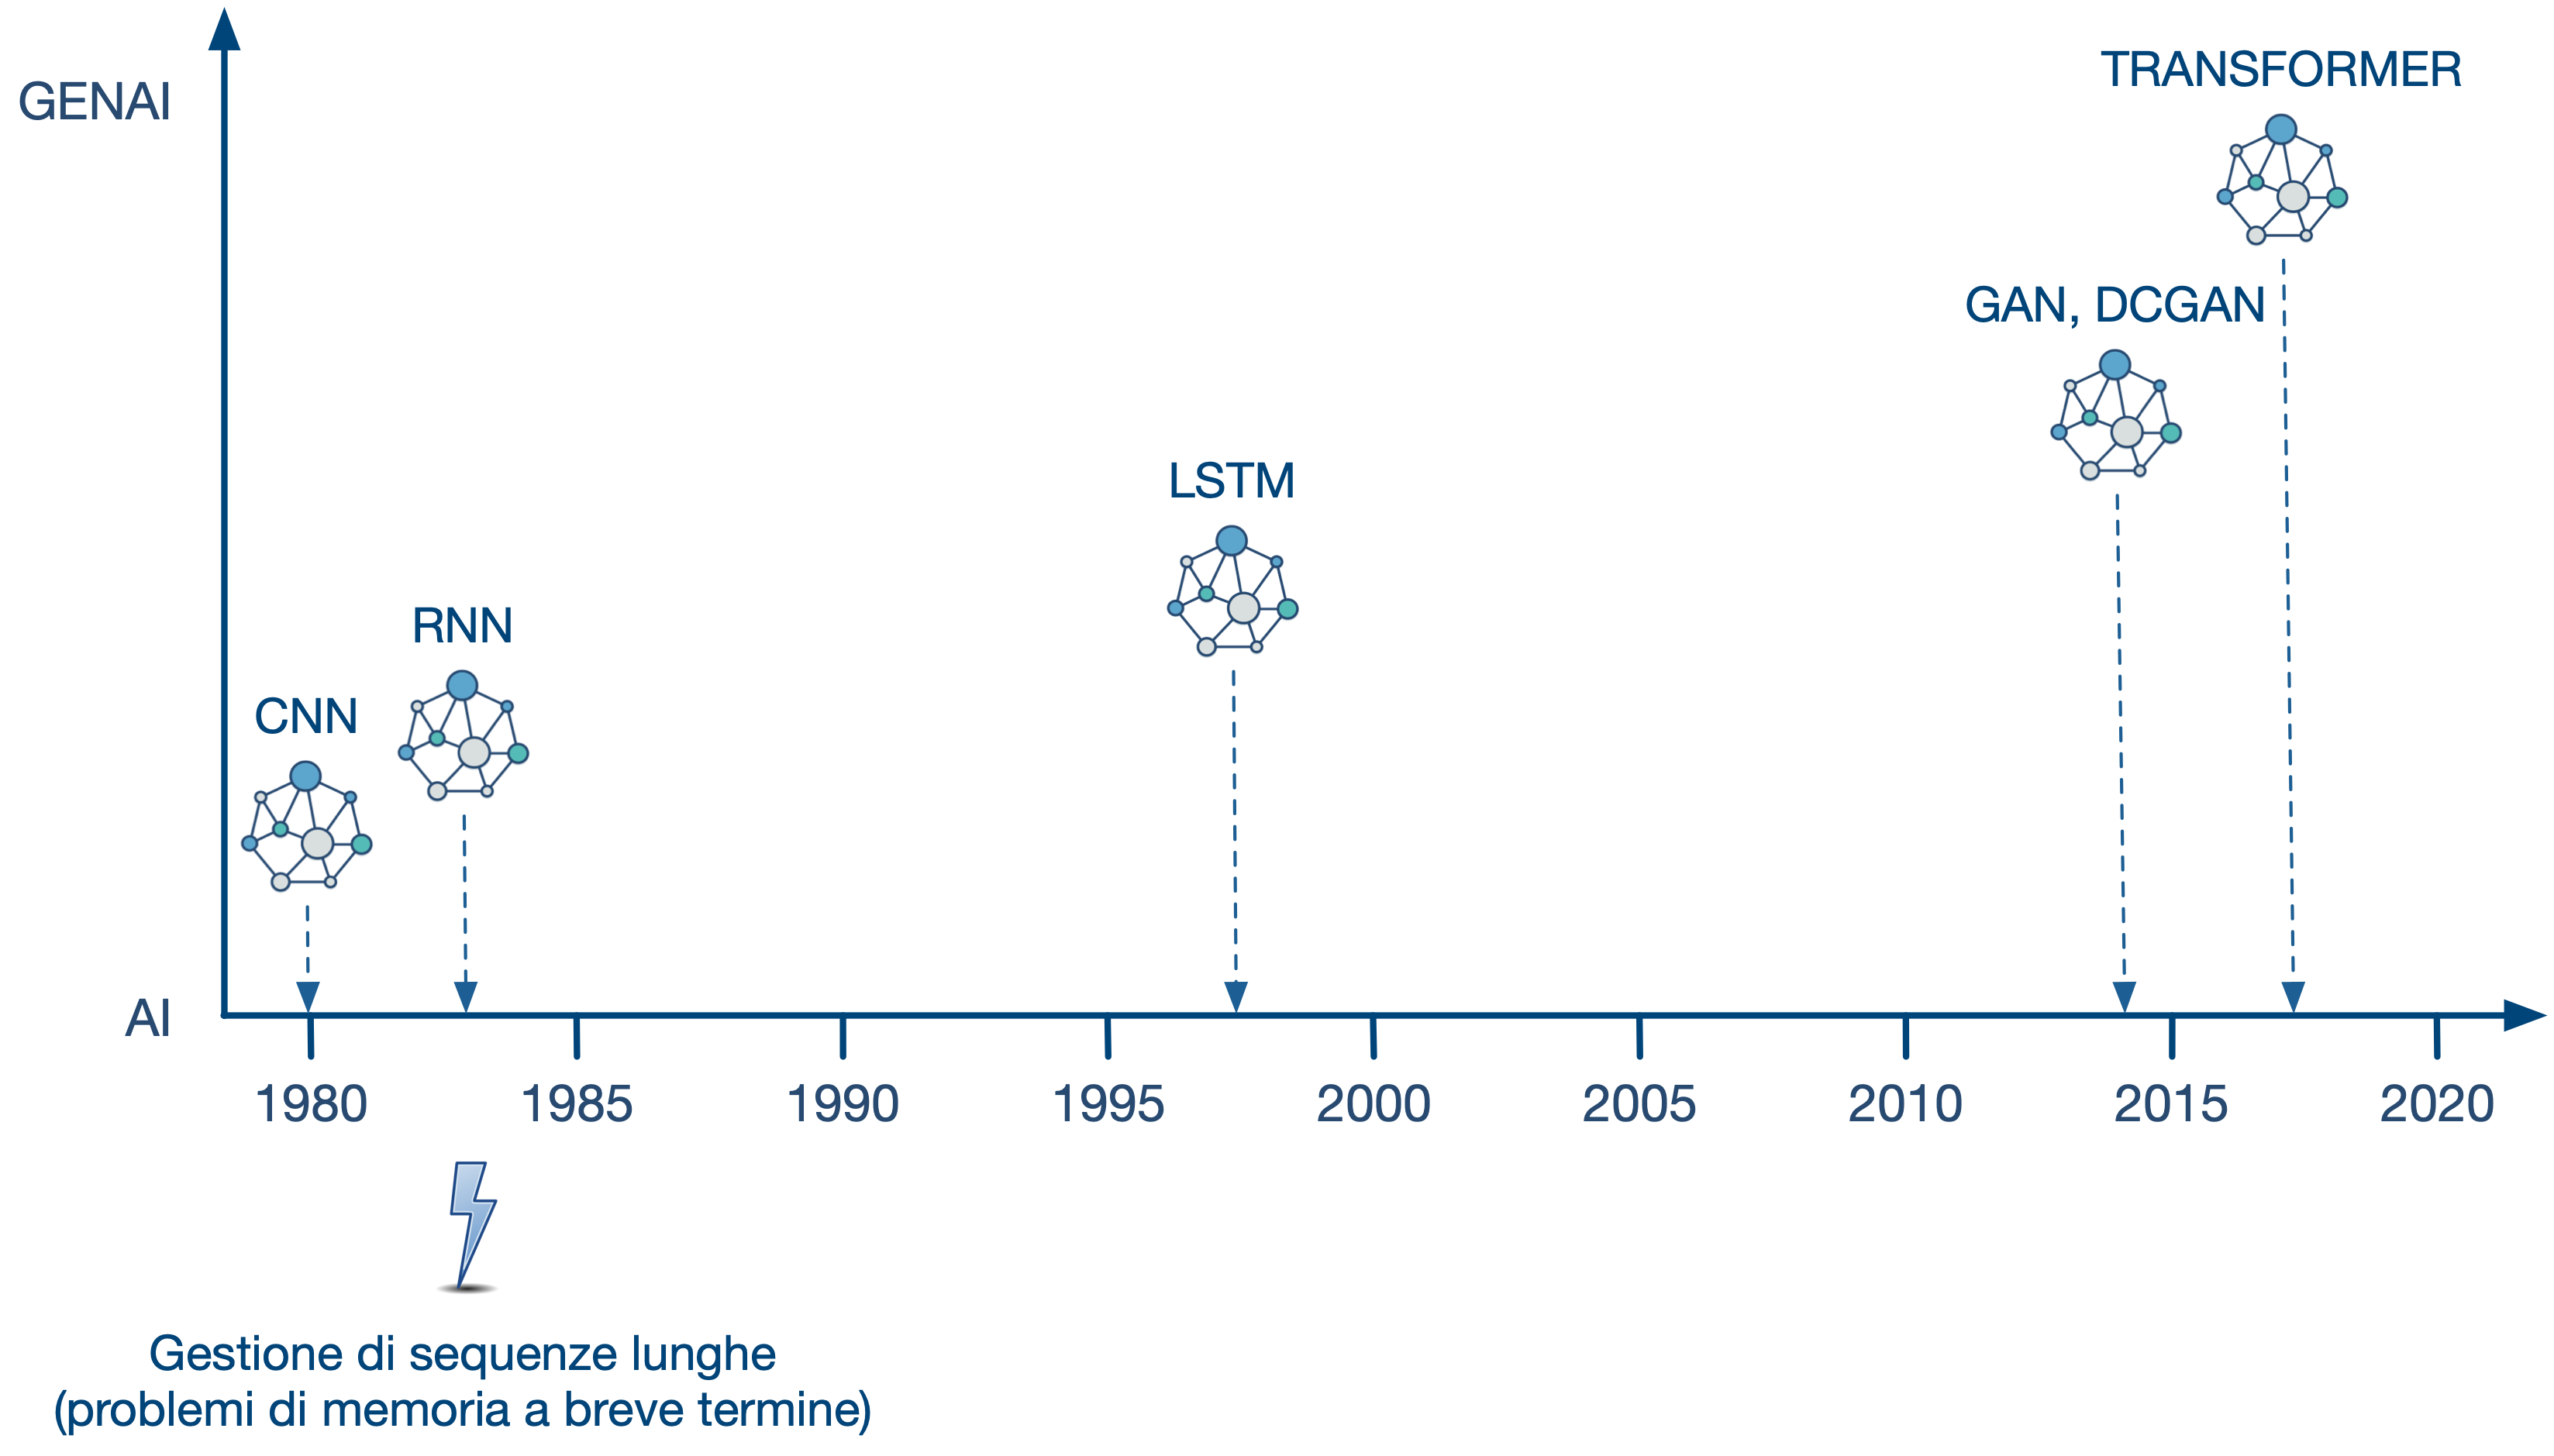
\includegraphics[width=\textwidth]{AI-GENAI-NLP-problems-2.png}
		\end{minipage}
	\end{figure}
}
	\only<4>{
	\begin{figure}[ht]
		\begin{minipage}[b]{0.95\linewidth}
			\centering
			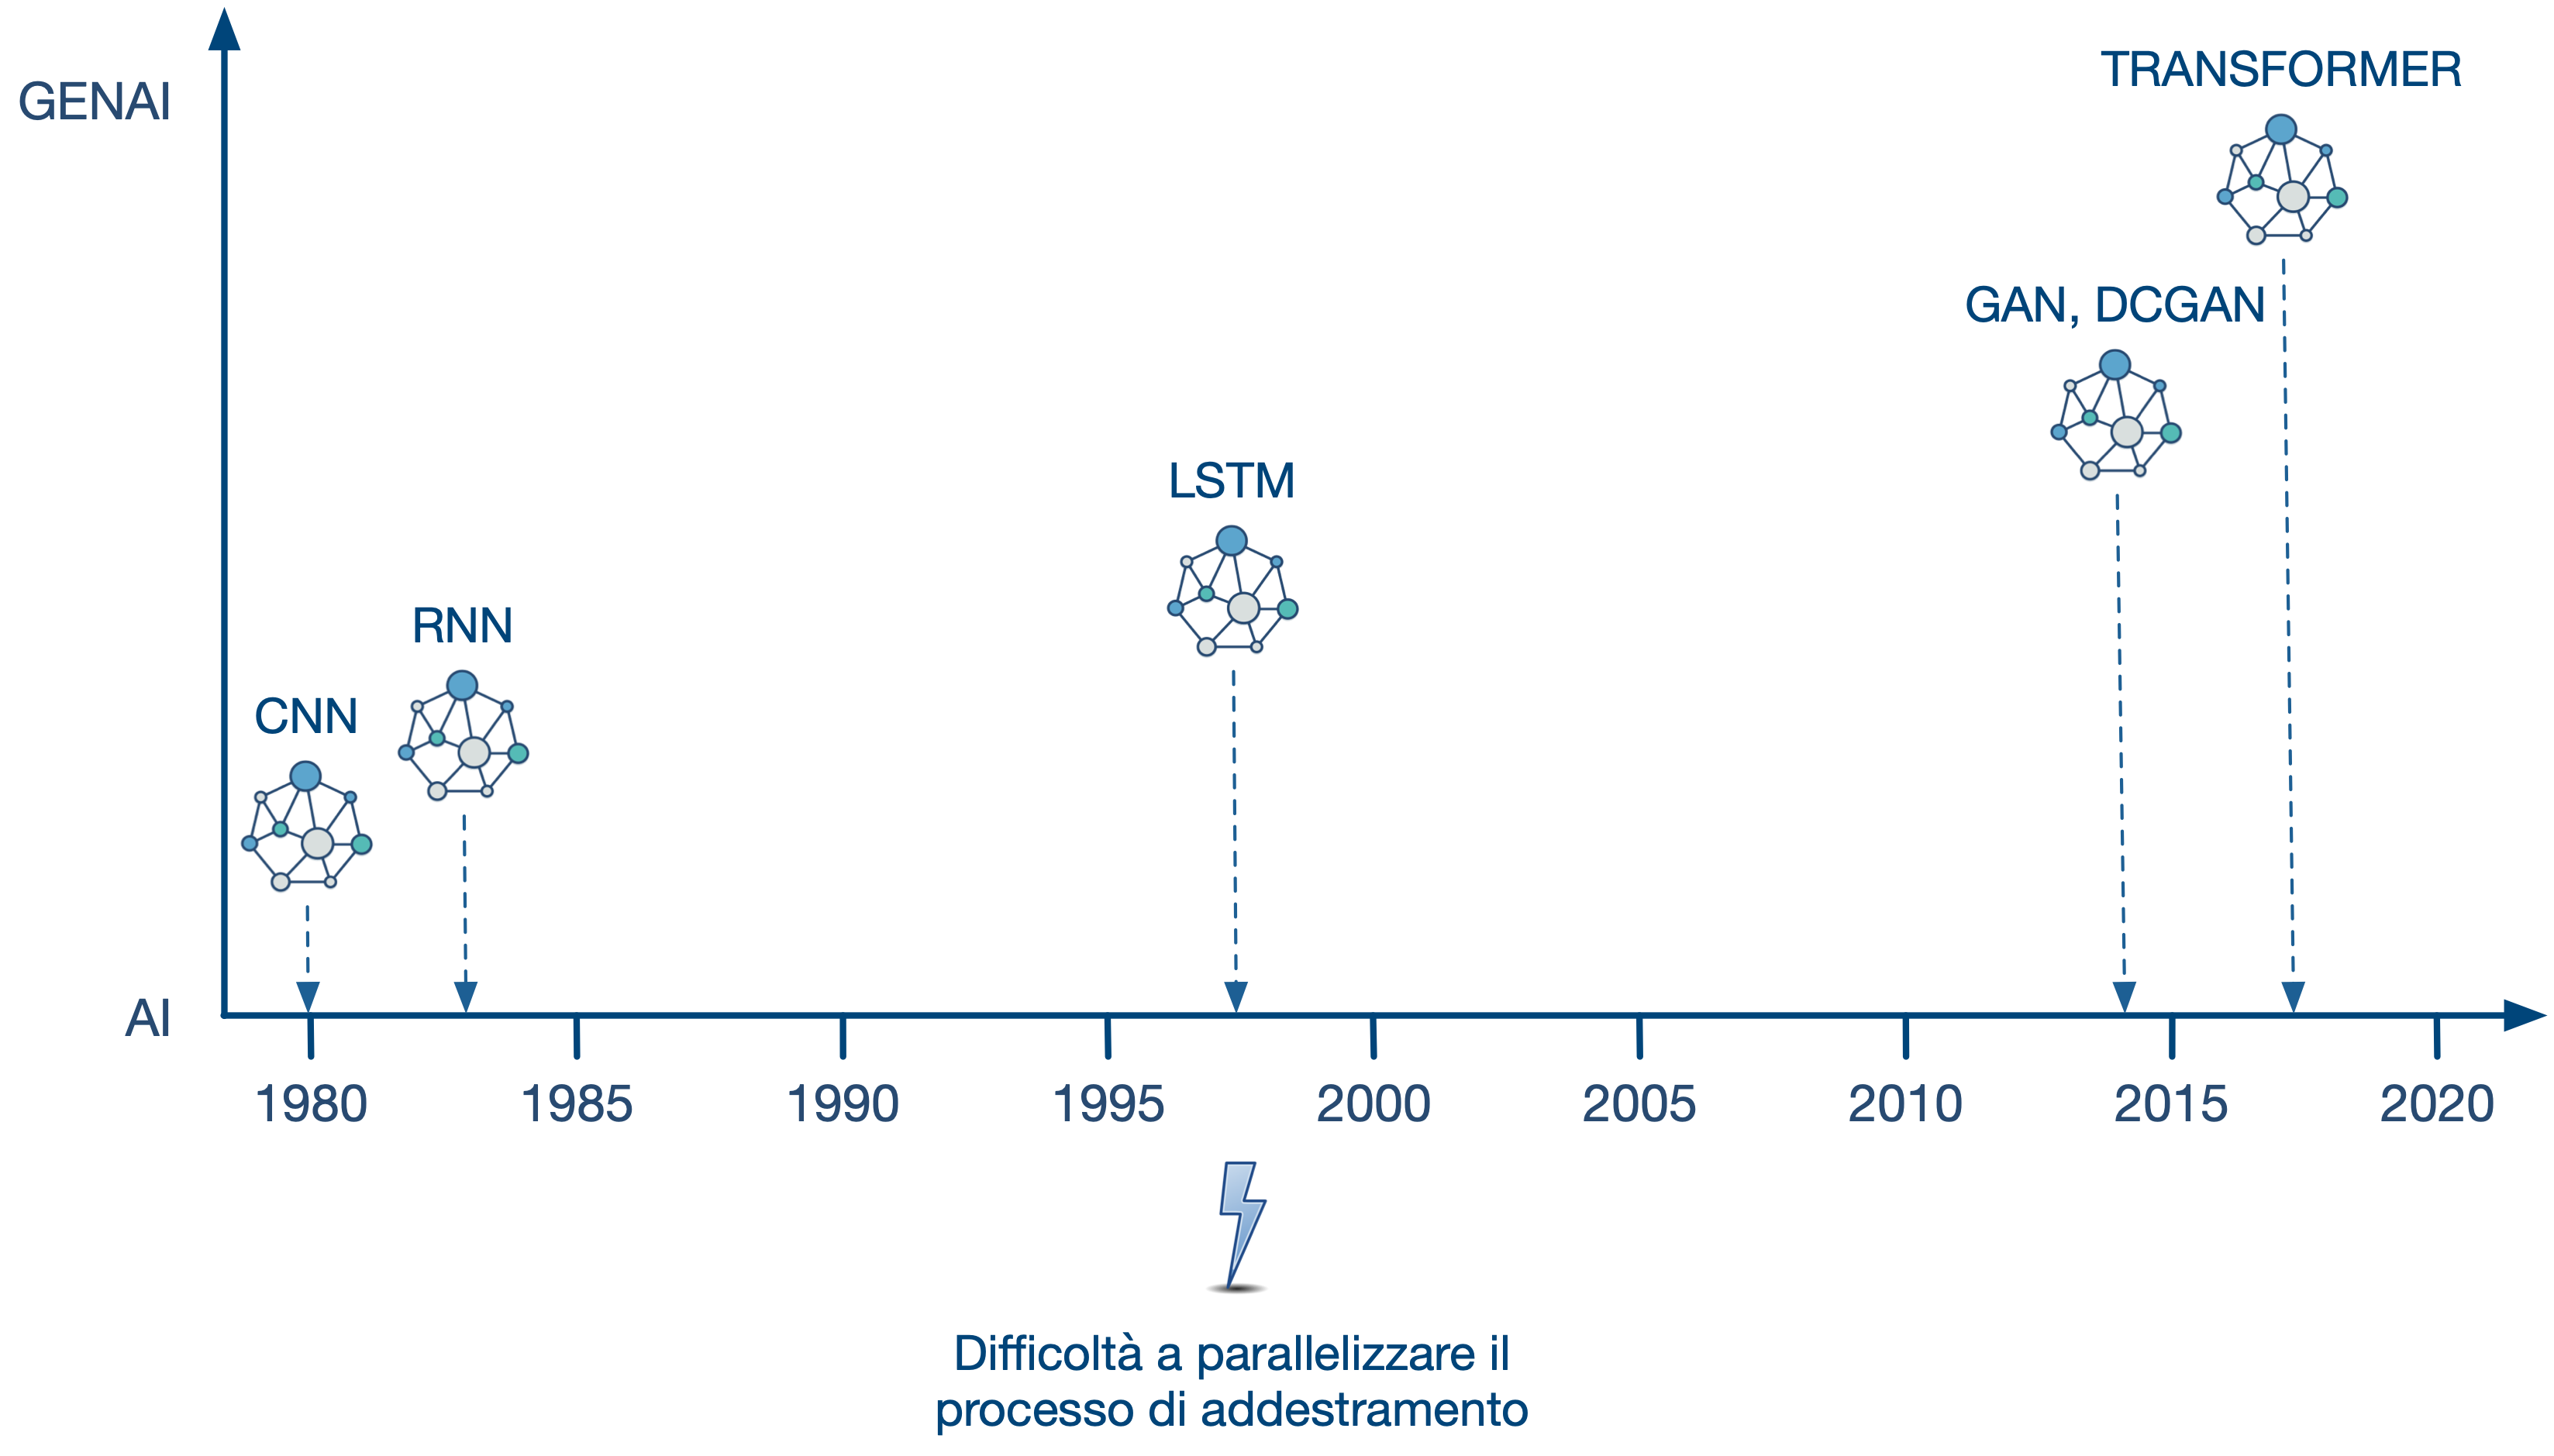
\includegraphics[width=\textwidth]{AI-GENAI-NLP-problems-3.png}
		\end{minipage}
	\end{figure}
}
	\only<5>{
	\begin{figure}[ht]
		\begin{minipage}[b]{0.95\linewidth}
			\centering
			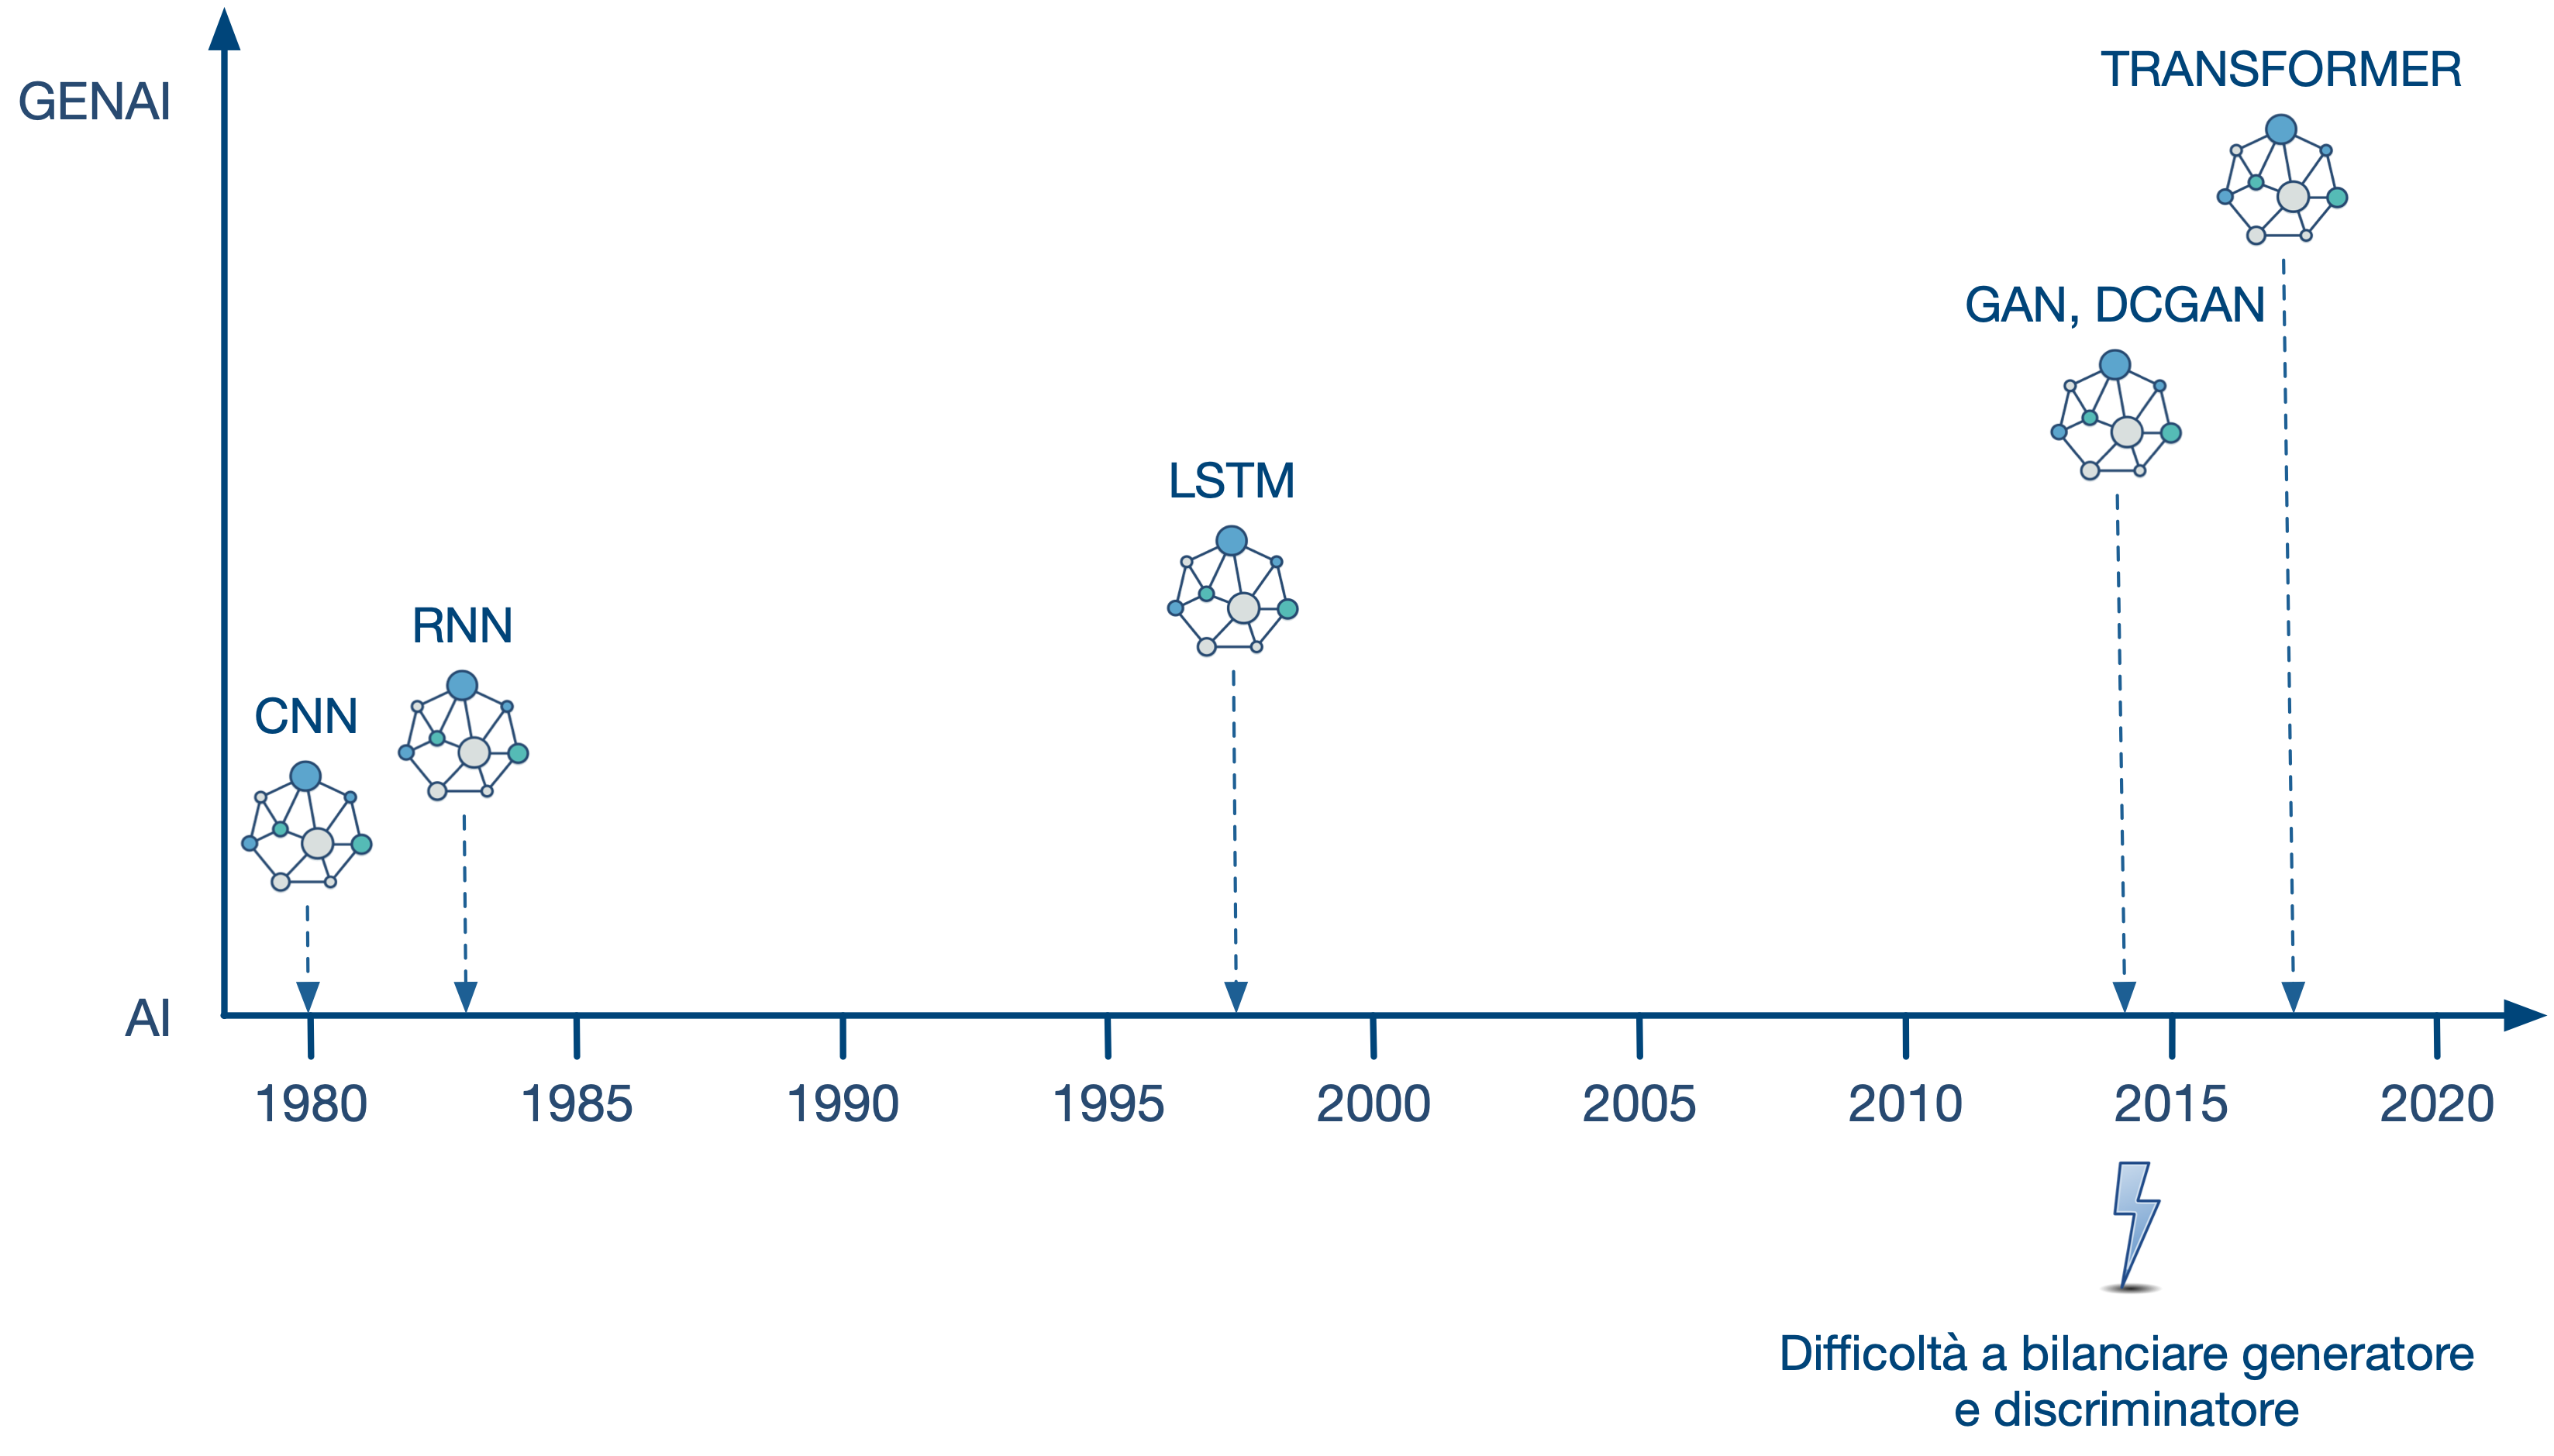
\includegraphics[width=\textwidth]{AI-GENAI-NLP-problems-4.png}
		\end{minipage}
	\end{figure}
}
}
\end{frame}
%
\begin{frame}[t] \frametitle{Architetture principali}
\framesubtitle{Transformer}
{\scriptsize
\onslide<1->
	\begin{minipage}[t]{\textwidth}
		\vspace*{-.5cm}
		\begin{figure}
			\centering
			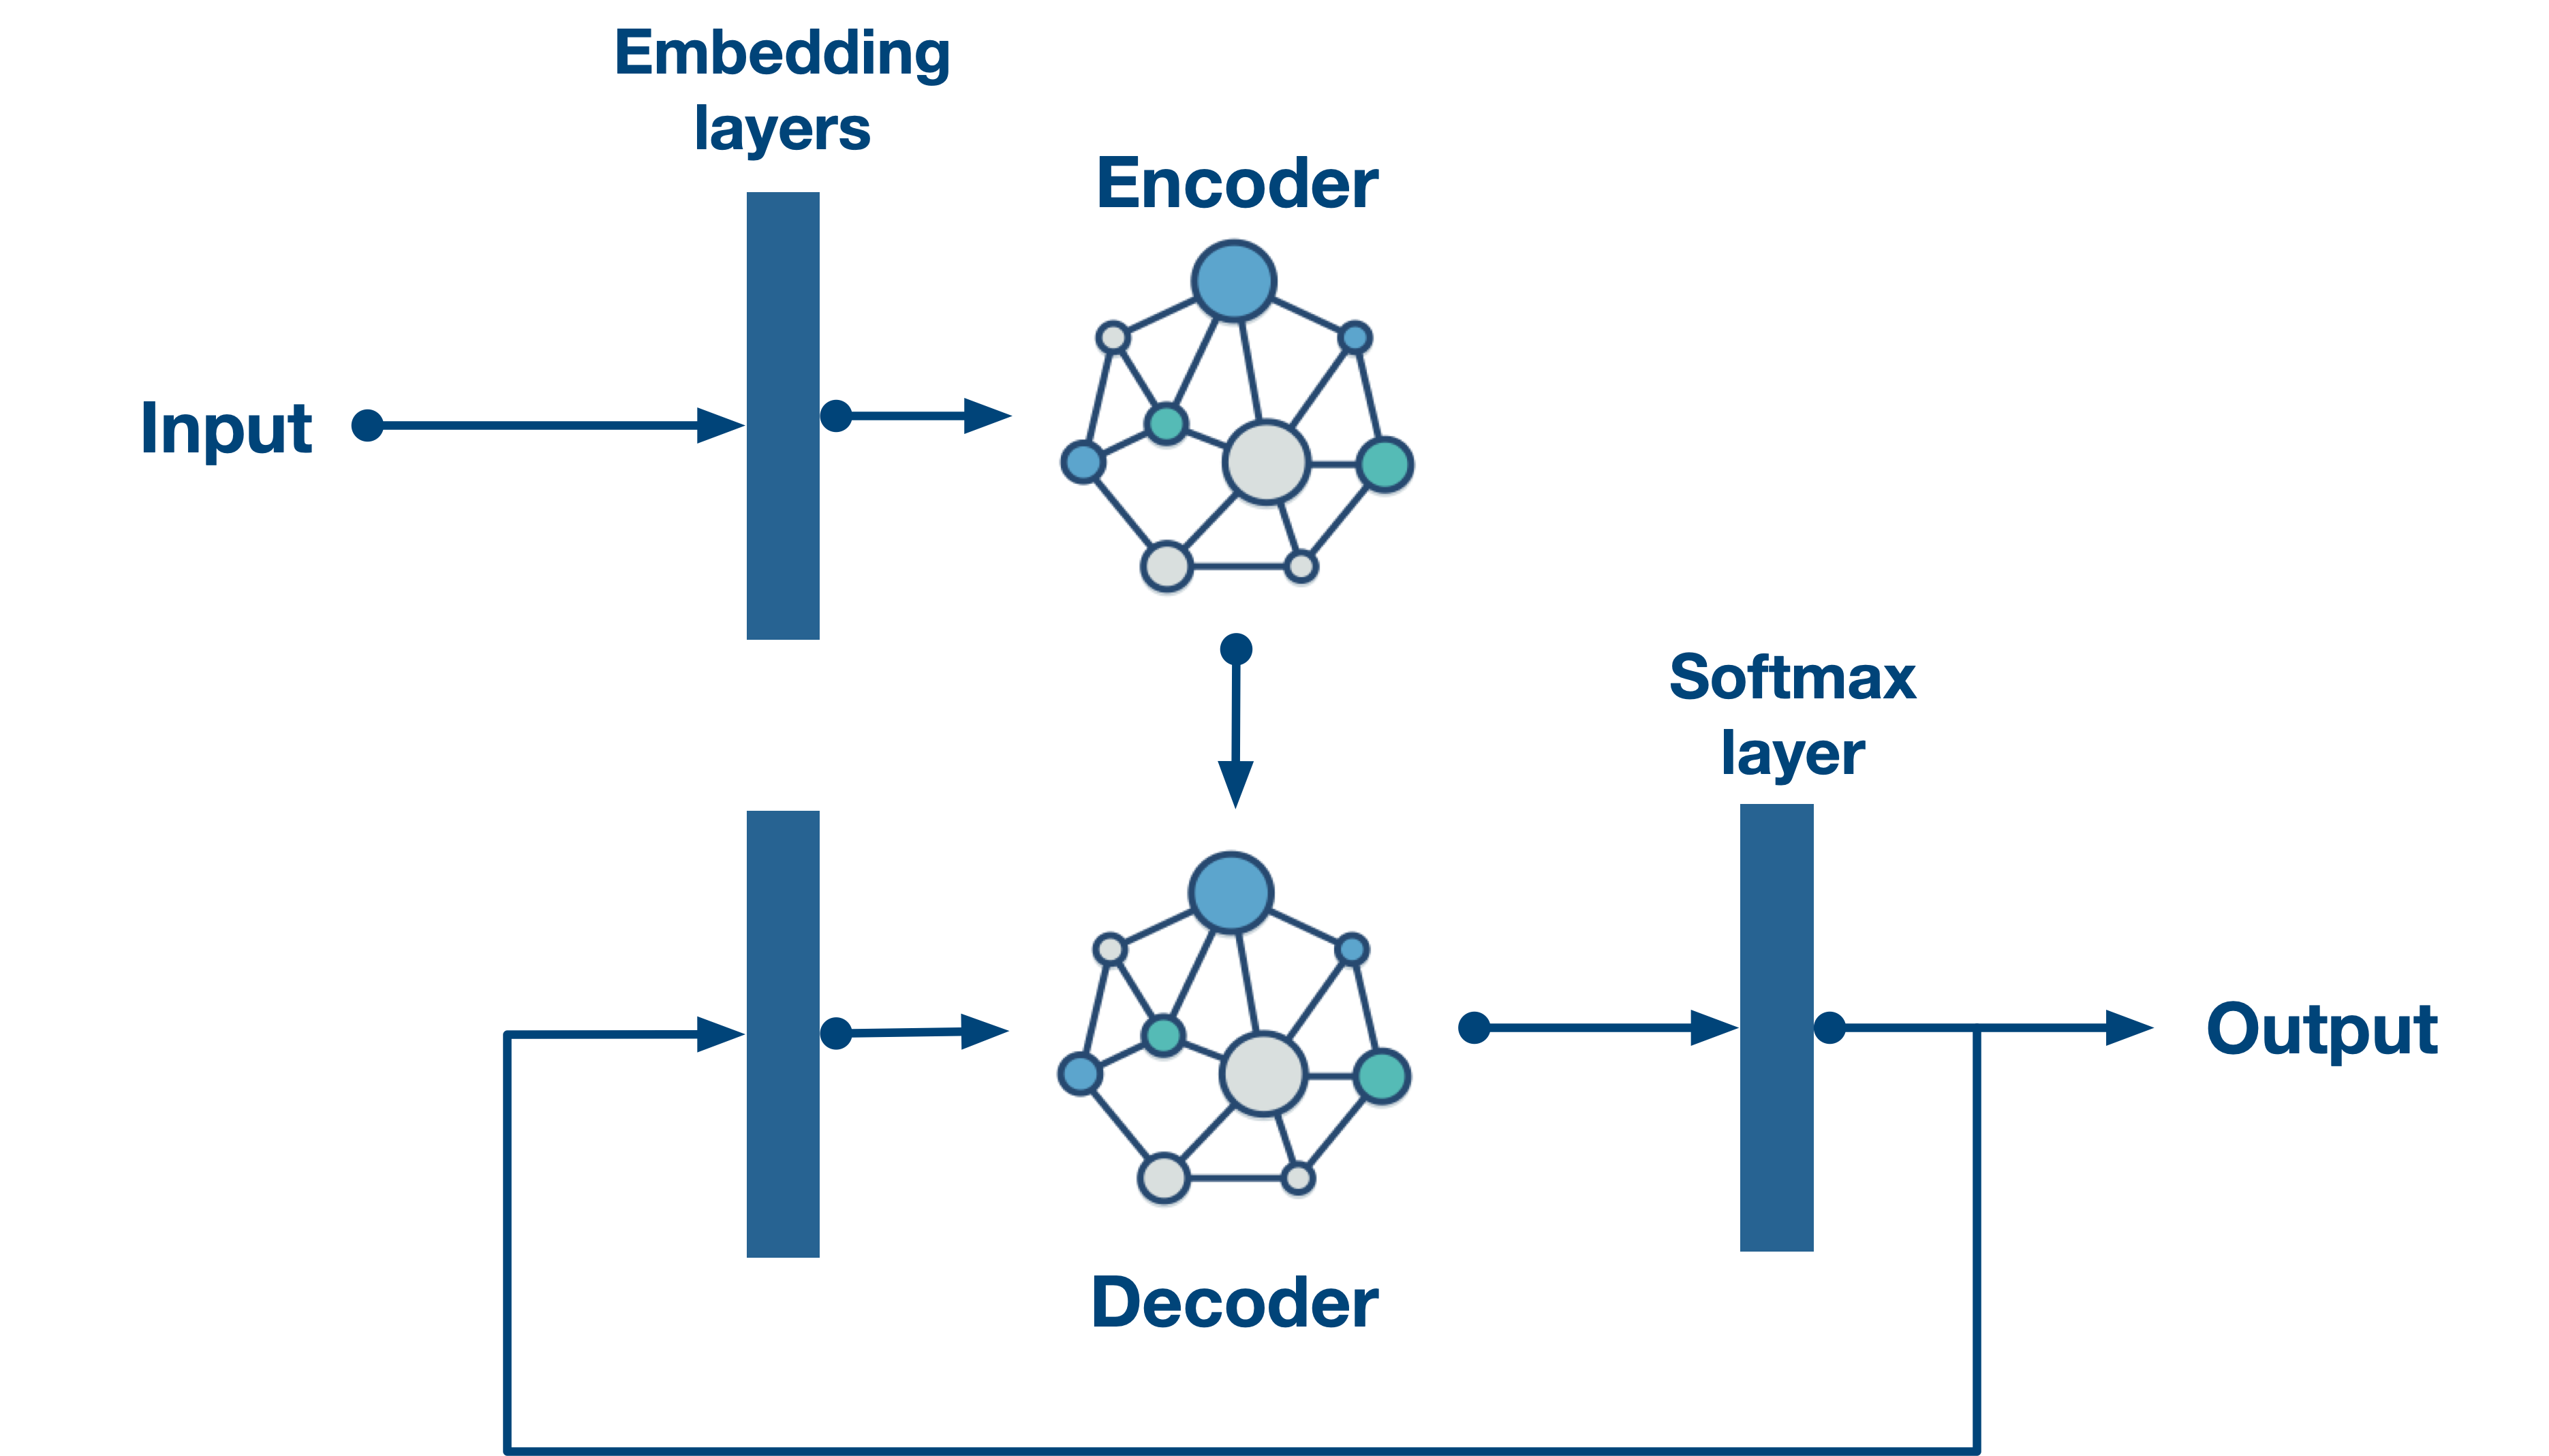
\includegraphics[width=.5\textwidth]{Transformer.png}
			\\Architettura \emph{Transformer}
		\end{figure}
	\end{minipage}
	\\\vspace*{.3cm}
	\begin{minipage}[t]{\textwidth}
		\begin{itemize}[leftmargin=10pt,align=right]
			\item[\alert{\faArrowCircleRight}] Nato come concetto algoritmico nel 2017
			\onslide<1->\item[\alert{\faArrowCircleRight}] Architettura rivoluzionaria rispetto a RNN ed LSTM
			\begin{itemize}[leftmargin=10pt,align=right]
				\onslide<2->\item[\alert{\faArrowCircleRight}] \alert{\emph{Encoder}}
				\begin{itemize}[leftmargin=10pt,align=right]
					\item[\alert{\faArrowCircleRight}] \alert{Obiettivo:} elaborare l'\emph{input} e generare rappresentazioni che catturano il suo significato
				\end{itemize}
				\onslide<3->\item[\alert{\faArrowCircleRight}] \alert{\emph{Decoder}}
				\begin{itemize}[leftmargin=10pt,align=right]
					\item[\alert{\faArrowCircleRight}] \alert{Obiettivo:} ottenere le rappresentazioni dell'\emph{encoder} come \alert{contesto} per generare l'\emph{output} (es. un testo)
				\end{itemize}
				\onslide<4->\item[\alert{\faArrowCircleRight}] \alert{\emph{Softmax layer}}
				\begin{itemize}[leftmargin=10pt,align=right]
					\item[\alert{\faArrowCircleRight}] \alert{Obiettivo:} restituire la scelta del \emph{decoder} reputata da lui più probabile
				\end{itemize}
			\end{itemize}
		\end{itemize}
	\end{minipage}
}
\end{frame}
%
\begin{frame}[t] \frametitle{Transformer}
\framesubtitle{Meccanismo di \emph{attention}}
{\scriptsize
\onslide<1->
	\begin{minipage}[t]{\textwidth}
		\vspace*{-.5cm}
		\begin{figure}
			\centering
			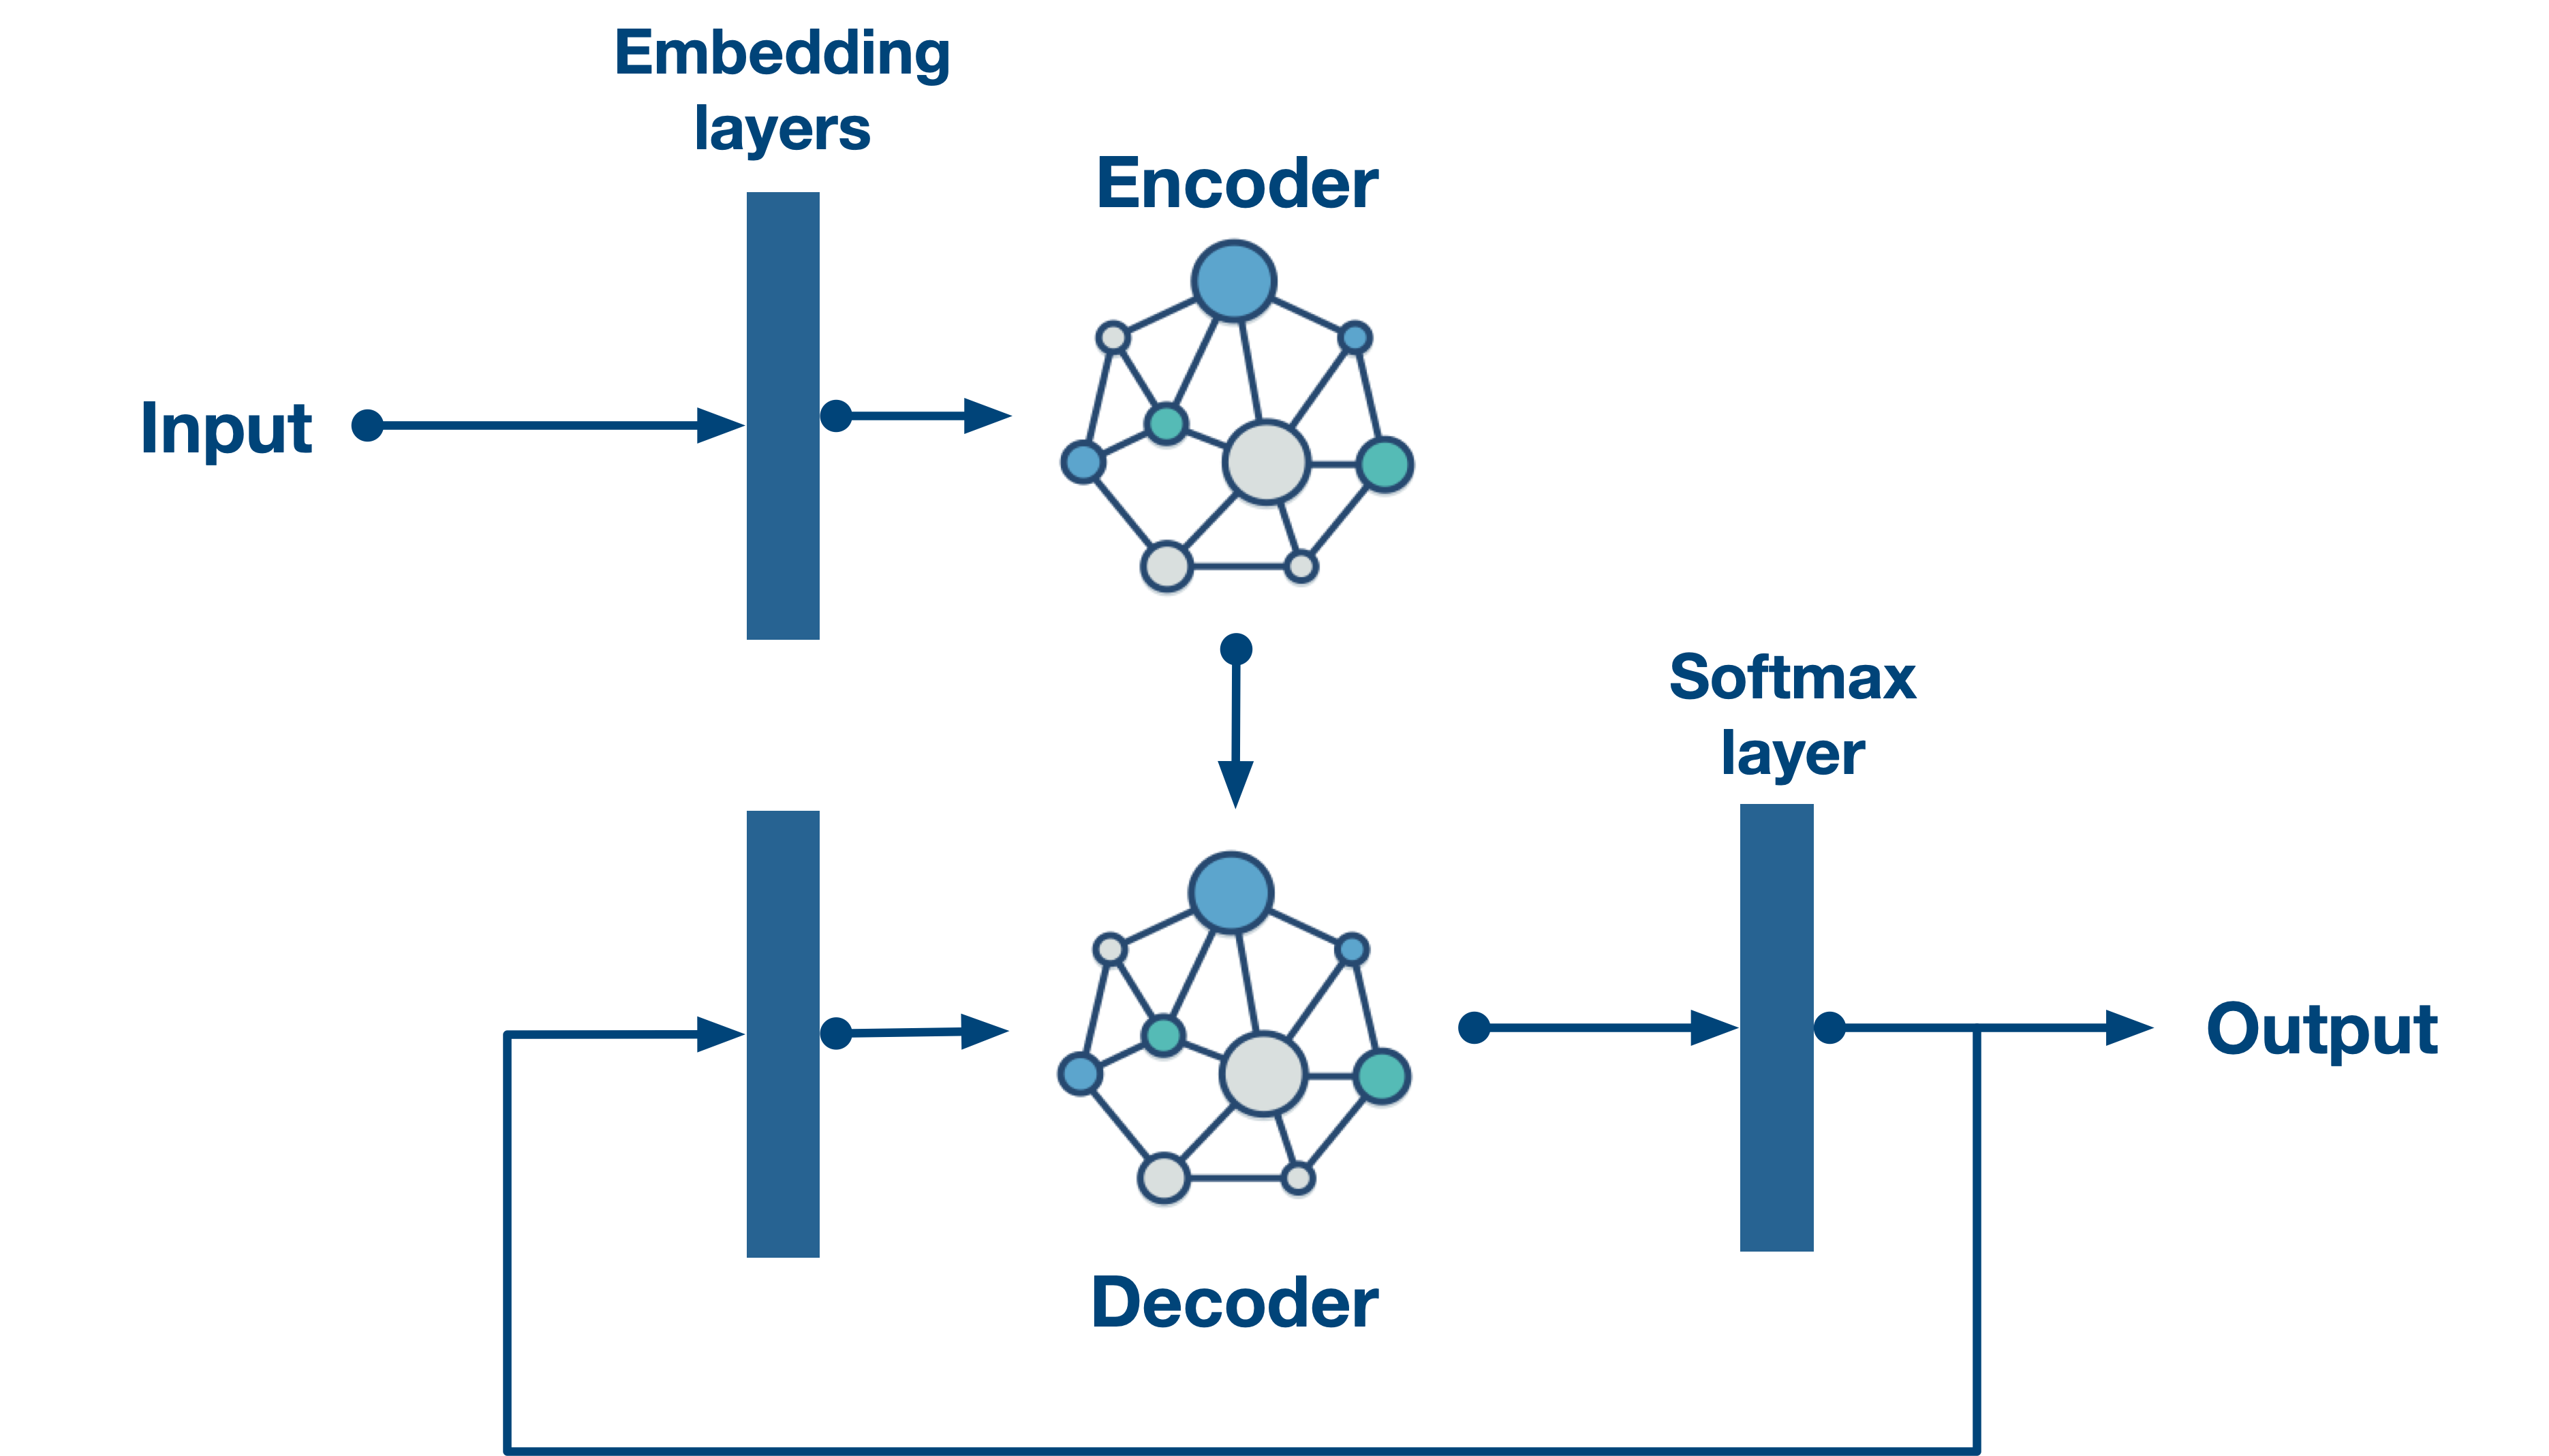
\includegraphics[width=.5\textwidth]{Transformer.png}
			\\Architettura \emph{Transformer}
		\end{figure}
	\end{minipage}
	\\\vspace*{.3cm}
	\begin{minipage}[t]{\textwidth}
		\begin{itemize}[leftmargin=10pt,align=right]
			\item[\alert{\faArrowCircleRight}] Prime strutture basate su Encoder-Decoder soffrivano di un problema di \emph{bottleneck}
			\begin{itemize}[leftmargin=10pt,align=right]
				\onslide<2->\item[\alert{\faArrowCircleRight}] Ultimo \emph{layer} nascosto dell'\emph{encoder} doveva modellare \alert{tutto} il contesto utilizzato dal \emph{decoder}
				\onslide<3->\item[\alert{\faArrowCircleRight}] \emph{Decoder} in stallo finché l'\emph{encoder} non finiva il suo lavoro
			\end{itemize}
			\onslide<4->\item[\alert{\faArrowCircleRight}] \alert{\emph{Attention}} come soluzione al problema
				\begin{itemize}[leftmargin=10pt,align=right]
					\onslide<5->\item[\alert{\faArrowCircleRight}] \emph{Decoder} ottiene informazione sul contesto da ciascun \emph{layer} nascosto dell'\emph{encoder}
					\onslide<6->\item[\alert{\faArrowCircleRight}] Gestione del contesto più efficace e persistente nel tempo
					\onslide<7->\item[\alert{\faArrowCircleRight}] Gestione dell'addestramento ad alto grado di parallelizzazione$\ldots$
					\onslide<8->\item[\alert{\faArrowCircleRight}] $\ldots$ quindi, su \emph{dataset} di addestramento \alert{estremamente grandi}
				\end{itemize}
		\end{itemize}
	\end{minipage}
}
\end{frame}
%